\cotefile{14}
\scanpage{87}
Relations entre hom. de V.A. et groupes de N.S.

\diagram{\begin{tikzcd}[ampersand replacement=\&,column sep=large,row sep=huge]
C^1(A) \arrow[r] \arrow[d]
 \& H^2(A)\otimes Q_\ell(1)=H^2(A,Q_\ell(1))=\bigwedge^2 H^1(A)\otimes Q_\ell(1)
   \arrow[d,"{\substack{\text{déduit de l'accouplement}\\ H^1(A)\times H^1(A^*)\to Q_\ell(\unsure{+1|-1})}}"] \\
\operatorname{Hom}(A,A^*) \arrow[r] \arrow[dr,"{\substack{\text{application}\\\text{``graphe'' (pas additive!)}}}"']
 \& \operatorname{Hom}(H^1(A^*),H^1(A)) \arrow[dr] \\
 \& C^n(A\times A^*) \arrow[r]
 \& H^{2n}(A\times A^*)\otimes Q_\ell(n)
\end{tikzcd}}

\[ (n=\dim A) \]

\[ \bar u=(\operatorname{id}_A,u) \]
\diagram{\begin{tikzcd}[ampersand replacement=\&]A\arrow[r]\&A\times A^*\end{tikzcd}}

\diagram{\begin{tikzcd}[ampersand replacement=\&,column sep=large,row sep=large]
H^{\unsure{\bullet}}(A) \arrow[r,"{\unsure{\bar u_*}}"] \& H^{\unsure{\bullet}}(A\times A^*)(..) \\
H^{\unsure{\bullet}}(A) \& H^{\unsure{\bullet}}(A\times A^*)\arrow[l,"{\deleted{\unsure{\bar u^*}}\,\unsure{\bar u^*}}"']
\end{tikzcd}
\qquad
\begin{tikzcd}[ampersand replacement=\&,column sep=large,row sep=small]
H^0(A) \arrow[r]\&H^{2n}(A\times A^*)(n)\\
\times \& \times\\
H^{2n}(A) \arrow[d,phantom,"{\unsure{\wr}}"] \& H^{2n}(A\times A^*)\arrow[l]\arrow[d,phantom,"{\unsure{\wr}}"]\\
Q_\ell(-n)\&Q_\ell(-n)
\end{tikzcd}}

\diagram{\begin{tikzcd}[ampersand replacement=\&,column sep=huge]
H^1(A)\&H^1(A\times A^*)=H^1(A)\times H^1(A^*)
\arrow[l,"{(\operatorname{id}_{H^1(A)},u^1)}"']
\end{tikzcd}}

\[ \unsure{\bar u_*(1)|\bar u_!(1)} \]

\margin{86}
\scanpage{88}
\margin{87}
\mspage{- 24 -}

\uline{Preuve} : Soit $G$ un faisceau $C'$-acyclique. Il suffit de montrer que pour tout objet $X$ de $C$,
\[
\check H^q(C^{\wedge}/X,\mathcal H^0(u_{\unsure{s}}(G)))=0\qquad q>0
\]

Il suffit donc de montrer que pour toute famille couvrante
$\mathcal U=(U_i\longrightarrow X,\ i\in I)$ dont l'existence est assurée par la condition (\unsure{CWC|CNC}),
$H^q(\mathcal U,\mathcal H^0(u_{\unsure{s}}(G)))=0\quad\inserted{\forall}\ q>0$.
Mais $u$, étant un foncteur continu, transforme la famille couvrante $\mathcal U$ en une famille couvrante de $u(X)$ ; et par définition du foncteur image directe, on a l'égalité :
\[
H^q(\mathcal U,\mathcal H^0(u_{\unsure{s}}(G)))=H^q(u(\mathcal U),\mathcal H^0(G))
\]
\margin{$\unsure{\forall\ \longrightarrow}$}
Le faisceau $G$ étant $C'$-acyclique, ces groupes sont nuls pour tout $q>0$. c.q.f.d.

La notion de faisceau $C$-acyclique n'est pas intrinsèque.
Elle ne dépend pas uniquement du topos $C^{\sim}$ défini par le site $C$, mais aussi du site particulier choisi pour définir le topos $C^{\sim}$ (3.11).
Nous allons maintenant définir une propriété intrinsèque.

\margin{\figure{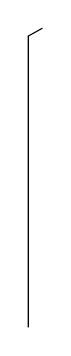
\begin{tikzpicture}[x=1cm,y=1cm]\draw (0.18,3.8)--(0,3.7)--(0,0);\end{tikzpicture}}}
\uline{Proposition 3.4} : Soient $E$ un topos annelé par un anneau $A$ de $E$, $F$ un $A$-Module. Les propriétés suivantes sont équivalentes :

i) Pour tout objet $S$ de $E$ :
\[
H^q(S,F)=0\qquad\inserted{\forall}\ q>0.
\]
\[\ldots/\ldots\]
\scanpage{89}
Un homomorphisme $u:A\longrightarrow B$ de V.A. est connu quand on connaît la classe de cohomologie associée à son graphe \unsure{dans|de} $A\times B$,
\deleted{la \unsure{coho.}} (i.e. si on la connaît \unsure{en tant} \unsure{que} dans le \unsure{ann.} cohomologique $\ell$-adique), car alors on connaît le \unsure{graphe|groupe} $\Gamma\inserted{{}\subset A\times B}$ de $u$ car $T_{Q_\ell}(\Gamma)\subset T_{Q_\ell}(A\times B)$ est alors connu.

\uline{\unsure{D}} $=$, une ss-V.A. de $A$ est connue quand on connaît sa classe de cohomologie.

L'``interprétation'' cohomologique de l'isom
\[
C^1(A\times B)/\deleted{\unsure{=}}\ C^1(A)\times C^1(B)\simeq\operatorname{Hom}(A,B^*)
\]
est bien \unsure{clair|claire}, via
\diagram{\begin{tikzcd}[ampersand replacement=\&,column sep=large,row sep=large]
\bigwedge^2(H^1(A)\times H^1(B))(1)/\bigwedge^2 H^1(A)(1)\times\bigwedge^2 H^1(B)(1)
\arrow[r,phantom,"{\simeq}"] \& H^1(A)\otimes H^1(B)(1)\arrow[d,phantom,"{\unsure{\wr}}"]\\
\&\operatorname{Hom}(T_\ell(A),T_\ell(B^*))
\end{tikzcd}}

\uline{Question} Prouver que pour qu'une \unsure{classe} de $H^1(A)\otimes H^1(B)(1)\subset H^2(A\times B)(1)$ soit algébrique

\margin{88}
\scanpage{90}
\margin{89}
\mspage{- 19 -}

\uline{Preuve} : Soit $R$ le crible engendré par les $(U_i\longrightarrow X)$. Le faisceau associé à $R$ est isomorphe au faisceau associé à $X$. On applique alors la proposition précédente et la formule (19).
\margin{\figure{\begin{tikzpicture}[x=1cm,y=1cm]\draw (0,0)--(0.4,0.05)--(0.4,0.3)--(1,0.4);\end{tikzpicture}}}
Cette suite spectrale est \deleted{due à}\inserted{celle de} Cartan-Leray.

\margin{\figure{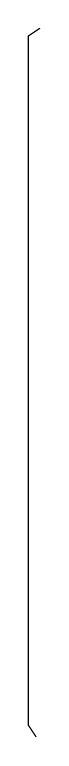
\begin{tikzpicture}[x=1cm,y=1cm]\draw (0.15,9)--(0,8.9)--(0,0.15)--(0.1,0);\end{tikzpicture}}}
\uline{Corollaire 2.5} : Il existe une suite spectrale fonctorielle en $F$ et en $X$ (objet de $C$) :
\[
H^{p+q}(C^{\sim}/X,F)\Longleftarrow\check H^p(X,\mathcal H^q(F))
\]
Cette suite spectrale fournit, lorsque $X$ varie dans $C$, la suite spectrale de préfaisceaux :
\[
\mathcal H^{p+q}(F)\Longleftarrow\check{\mathcal H}^{p}(\mathcal H^q(F))
\]
Ces suites spectrales fournissent des morphismes fonctoriels :
\margin{$\unsure{\checkmark}$}
\[
\Phi^q(F):\check{\mathcal H}^{q}(\mathcal H^0(F))\longrightarrow\mathcal H^q(F)
\]
\[
\Phi_X^q(F):\check H^q(\unsure{E|S}\ X,\mathcal H^0(F))\longrightarrow H^q(X,F)
\]
Les morphismes $\Phi^q$ et $\Phi_X^q$ sont des isomorphismes lorsque $q$ égale $0$ ou $1$. Les morphismes $\Phi^2$ et $\Phi_X^2$ sont des monomorphismes.

Plus généralement, lorsque les préfaisceaux $\mathcal H^i(F)$ sont nuls pour $0<i<n$, les morphismes $\Phi^q(F)$ et $\Phi_X^q(F)$ sont des isomorphismes pour $0\leq q\leq n$ et des monomorphismes pour $q=n+1$.

\uline{Preuve} : La première suite spectrale s'obtient en passant à la limite inductive dans la suite spectrale de la proposition 2.3 sur les
\[\ldots/\ldots\]
\scanpage{91}
\begin{flushright}
Tableau des\\
classes de cycles \ldots
\end{flushright}

\margin{90}
\scanpage{92}
Anneaux de classes de cycles\\
sur une variété projective non singulière\\
sur un corps $k$ alg. clos

\diagram{\begin{tikzcd}[ampersand replacement=\&,
 column sep=1.2cm,row sep=1.25cm,
 execute at end picture={
  \draw ([xshift=-0.5cm,yshift=0.45cm]anum.north west) rectangle ([xshift=0.45cm,yshift=-0.45cm]az.south east);
  \draw ([xshift=-0.45cm,yshift=0.4cm]apic.north west) rectangle ([xshift=1.8cm,yshift=-0.45cm]alin.south east);
  \draw[->] (discrete.west) -- ([xshift=0.45cm,yshift=0.25cm]aq.north east);
  \draw[->] (continuous.west) -- ([xshift=1.8cm]alin.east);
  \draw ([xshift=-0.35cm]anum.south west) .. controls ([xshift=-0.65cm]anum.south west) and ([xshift=-0.3cm,yshift=0.4cm]atau.west) .. ([xshift=-0.65cm,yshift=0.6cm]atau.west)
        .. controls ([xshift=-0.3cm,yshift=0.3cm]atau.west) and ([xshift=-0.65cm]atau.west) .. (atau.west);
  \node[anchor=east,align=left] at ([xshift=-0.7cm,yshift=0.6cm]atau.west) {groupe libre\\de type fini?};
  \draw (atau.south west) .. controls ([xshift=-0.55cm]atau.south west) and ([xshift=-0.3cm,yshift=0.5cm]aalg.west) .. ([xshift=-0.65cm,yshift=0.7cm]aalg.west)
        .. controls ([xshift=-0.3cm,yshift=0.3cm]aalg.west) and ([xshift=-0.55cm]aalg.west) .. (aalg.west);
  \node[anchor=east] at ([xshift=-0.7cm,yshift=0.7cm]aalg.west) {Groupe fini?};
  \draw (aalg.south west) .. controls ([xshift=-0.4cm]aalg.south west) and ([xshift=-0.2cm,yshift=0.5cm]apic.west) .. ([xshift=-0.55cm,yshift=0.7cm]apic.west)
        .. controls ([xshift=-0.2cm,yshift=0.3cm]apic.west) and ([xshift=-0.4cm]apic.west) .. (apic.west);
  \node[anchor=east] at ([xshift=-0.6cm,yshift=0.7cm]apic.west) {V.A.?};
  \draw ([xshift=-0.3cm,yshift=0.3cm]oldq.north west)--([xshift=0.35cm,yshift=-0.4cm]oldz.south east);
  \draw ([xshift=0.2cm,yshift=0.35cm]oldq.north east)--([xshift=-0.3cm,yshift=-0.3cm]oldz.south west);
  \draw (car.west)--(az.north west);
  \draw ([yshift=-0.3cm]ck.south west) .. controls ([yshift=-0.5cm]ck.south west) and ([xshift=-0.15cm,yshift=-0.35cm]ck.south) .. ([yshift=-0.55cm]ck.south)
        .. controls ([xshift=0.15cm,yshift=-0.35cm]ck.south) and ([yshift=-0.5cm]ck.south east) .. ([yshift=-0.3cm]ck.south east);
  \node[anchor=north,align=left] at ([yshift=-0.65cm]ck.south) {flèches\\qui sont des\\isom mod torsion};
  \draw ([xshift=-0.25cm,yshift=-0.45cm]alin.south west) .. controls ([yshift=-0.65cm]alin.south west) and ([xshift=0.25cm,yshift=-0.45cm]alin.south) .. ([xshift=0.45cm,yshift=-0.7cm]alin.south)
        .. controls ([xshift=0.6cm,yshift=-0.45cm]alin.south) and ([xshift=1.65cm,yshift=-0.65cm]alin.south) .. ([xshift=1.65cm,yshift=-0.45cm]alin.south);
  \node[anchor=north,align=left] at ([xshift=0.7cm,yshift=-0.8cm]alin.south) {flèches toutes\\surjectives};
 }]
 \& |[alias=anum]| A_{\mathrm{num}} \&\&\& |[alias=discrete]|\text{théorie discrète.}\\
 \& |[alias=atau]| A_\tau \arrow[u,"{?\ \unsure{\wr}}"']\arrow[r,"{\overset{!}{\sim}}"]
 \& |[alias=aq]|A_{Q_\ell\text{-hom}} \arrow[r]
 \& |[alias=oldq]|\deleted{\unsure{A_{Q_\ell\text{-hom}}}}
 \& |[alias=car,align=left]|\ensuremath{\substack{\text{\textcircled{car. 0}}\\\text{\unsure{en remplaçant}}\\\text{\unsure{théorie sing. entière.}}}}\\
 \& |[alias=aalg]| A_{\mathrm{alg}}\arrow[u]\arrow[r,"{\overset{?}{\sim}\ \textcircled{\unsure{t0|th0}}}"]
 \& |[alias=az]| A_{\unsure{\wedge Z_\ell|\widehat Z_\ell}\text{-hom}}\arrow[u]\arrow[r]
 \& |[alias=oldz]|\deleted{\unsure{A_{Z_\ell\text{-hom}}}}\arrow[u]\\
 |[alias=gtop]| G_{\mathrm{top}}K\arrow[uur,bend left=55]\arrow[urr,dashed,"?",bend right=10]
 \& |[alias=apic]| A_{\mathrm{pic}}\arrow[u]\\
 \& A_{\mathrm{alb}}\arrow[u,"{\unsure{\wr}\ ?}"]\\
 G_{\mathrm{alg}}K\arrow[uu]
 \& |[alias=alin]| A_{\mathrm{lin}}\arrow[u,"{\unsure{\wr}\ ?}"]\arrow[uul,"{\text{surj}}"']
 \&\& |[alias=continuous]|\text{théorie continue}\\
 |[alias=ck]| CK\arrow[u,"{\text{surj}}"']\arrow[ur]
\end{tikzcd}}

\margin{Autres équivalences : l'équivalence \unsure{régulière|rigide} $r$ et l'équivalence de Weil $\unsure{wh|w_h}$ et $W$ définis par Liebermann \ldots\ldots}

\margin{91}
\scanpage{93}
\begin{flushright}
Mumford-Nakai\\
Cycles algébriques\\
amples ....
\end{flushright}

\margin{92}
\scanpage{94}
\margin{\figure{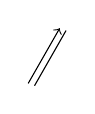
\begin{tikzpicture}[x=1cm,y=1cm]\draw[->](0,0)--(.4,.7);\draw(.08,-.03)--(.48,.67);\end{tikzpicture}} N.B. le critère implique \unsure{la condition|le critère} d'amplitude de A. Weil ....}

\uline{Th de Mumford-Nakai}\qquad $X$ schéma projectif sur corps $k$,
$L$ faisceau inv. sur $X$. Conditions équivalentes :

a) $L$ ample

b) Pour $\forall$ \deleted{sous-préschéma fermé intègre $Z$ de $X$}\inserted{faisceau cohérent $F$ sur $X$} \deleted{\unsure{de dim}} $\dim\operatorname{supp}F\geq1$, on a
\[
\chi(F\otimes L^{\otimes n})\longrightarrow+\infty\qquad\text{si }n\longrightarrow+\infty.
\]

b') Comme b), avec $F$ de la forme $\mathcal O_Z$, $Z$ un sous-préschéma intègre de $X$ de $\dim\geq1$.
\margin{on peut se borner à \uline{supposer}}

\unsure{b''}) Pour $\forall$ sous-préschéma intègre $Z$ de $X$, tels que $\dim Z=1$ (resp. $\dim Z\geq2$), il existe un entier $n=n_Z>0$ tel que
\[
\chi(L^{\otimes n}\otimes\mathcal O_Z)\geq2
\]
(resp. $\chi(L^{\otimes n}\otimes\mathcal O_Z)\geq1$).

c) Comme b), \uline{en remplaçant $\chi$ par} \deleted{\unsure{H}} $\dim H^0$

c') Comme b')

c'') Pour $\forall$ sous-préschéma intègre $Z$ de $X$ \inserted{$\boxed{\text{tels que }\dim Z=1\ (\dim Z\geq\unsure{1|2})}$} existe un entier $n=n_Z>0$ tel que
\[
\dim H^0(Z,L^{\otimes n}\otimes\mathcal O_Z)\geq2
\]
(resp. $\geq1$).

\margin{\uline{Critère numérique} ($X$ \unsure{irred} de dim $d$)
\[
\left\{\begin{array}{l}
D.C>0\quad\text{si }C\text{ courbe \unsure{irred}}\ \deleted{\unsure{de X}}\ >0\\
D^d>0
\end{array}\right.
\]
(\unsure{intersections} \unsure{calculées|calculés} dans $CK(X)$!)}

\deleted{d) Il existe un entier $\unsure{n|\nu}>0$ tel que $L^{\otimes\unsure{n|\nu}}$ admette une section\inserted{${}\neq0$}; et pour tout sous-préschéma intègre $Z$ de $X$, \deleted{il existe un}\inserted{\uline{de dim 1}}, il existe un entier $n>0$ tel que
\[
\dim H^0(Z,\unsure{L^{\otimes n}_{\otimes\mathcal O_Z}|L^{\otimes n}\otimes\mathcal O_Z})\geq2.
\]}

\deleted{d') \deleted{Pour} Il existe un entier $n>0$ tel que $L^{\otimes n}$ admette une section\inserted{${}\neq0$}, et pour $\forall$ sous-préschéma intègre $Z$ de $X$, de dim 1, on a $\deg(\unsure{L\otimes\mathcal O_Z|L\vert_Z})>0$.}

\margin{93\quad$\unsure{\xi}\,1$}
\scanpage{95}
$a)\Longrightarrow(b)+c))$ bien connu (on peut supposer $L$ très ample, et on applique la théorie du \unsure{pol.} de Hilbert)

$b)\Longrightarrow b')\Longrightarrow b'')$ trivial

$c)\Longrightarrow c')\Longrightarrow c'')$ trivial

On prouve les autres assertions par récurrence sur \deleted{\unsure{Hyp.}} $\dim X=d$, cela est trivial si $d=0$, et bien connu si $d=1$. Supposons $d\geq2$

$b'')\Longrightarrow\unsure{c''|d''})$ Grâce au

\uline{Lemme 1} Si les \deleted{conditions b''), $\exists n=n_0>0$}\inserted{restrictions de $\underline L$ aux sous-préschémas \inserted{intègres}} $Z$ de $X$ de dim $<d$ sont amples, alors $\exists n_0$ tel que
\[
n\geq n_0\Longrightarrow H^i(X,L^{\otimes n})=0\quad\text{pour }i\geq2
\]
\deleted{\unsure{tel que}}

\margin{\unsure{par des restrictions aux diviseurs} Mais il faut supposer $X$ \unsure{projective|projectif}}

cf lettre de Mumford.

\deleted{$d)\Longrightarrow c)$ trivial}

\deleted{$d)\Longleftrightarrow d')$ d'après le cas déjà \deleted{\unsure{traité}}\inserted{connu} $d=1$}

$\unsure{c''|d''})\Longrightarrow a)$ On peut supposer (via : EGA III \ldots) que $X$ est intègre. \deleted{\illegible{1}} \unsure{Soit} \deleted{\unsure{f}} $f$ une section de $\underline L^{\otimes n}$, \deleted{\unsure{on}} $D$ l'un de ses zéros, alors $D\neq\varnothing$ car $\underline L$ n'est pas trivial, donc $\dim D=d-1$. On \unsure{prouve}

\uline{Lemme 2} Sous les conditions du lemme 1, supposons \inserted{$\exists n>0$ tel} que $\underline L^{\otimes n}$ ait une section. Alors \deleted{$\unsure{\exists}$} $\exists n_0$ tel que
\[
n\geq n_0\Longrightarrow X\xrightarrow{\unsure{!}}\mathbf P H^0(X,L^{\otimes n})\quad\text{partout définie}
\]
et non \unsure{constant|constante}

\margin{$d\geq2$}

cf lettre Mumford ....

\uline{Questions} Dans l'énoncé d) et d') peut-on supprimer l'hyp d'existence d'une section $\neq0$ ?? \deleted{Oui si \illegible{1}}

\deleted{\unsure{dans}} Peut-on supprimer l'hyp. que $X$ projectif ??

\margin{94}
\scanpage{96}
\diagram{\begin{array}{ccccc}
\mathring P^{\unsure{+|\#}}&\subset&P^{\unsure{+|\#}}&\subset&\overline{P^{\unsure{+|\#}}}\\
\cup&&&&\cup\\
\mathring Q^{\unsure{+|\#}}&\subset&Q^+&=&\overline{Q^{\unsure{+|\#}}}\\
\cup&&&&\cup\\
\mathring{\overline R}&=&R&\subset&\overline R
\end{array}}

\[\boxed{\mathring Q^{\unsure{+|\#}}\subset P^{\unsure{+|\#}}}\quad
\text{d'où}\quad Q^{\unsure{+|\#}}=\overline{Q^{\unsure{+|\#}}}\subset\overline{P^{\unsure{+|\#}}}\]
\margin{\uline{Prop} de \uline{\unsure{Cauchy|Castel.}}}
\[\left(\text{donc }\mathring Q^{\unsure{+|\#}}\subset\mathring{\overline{P^{\unsure{+|\#}}}}=\mathring P^{\unsure{+|\#}}\right)\]
d'où par polarité, comme $Q^+=Q^{+0}$
\[\overline{P^{\unsure{+|\#}}}^{\,0}=P^{\unsure{+|\#}0}\subset Q^{\unsure{+|\#}}.\]

\[P^+\ni x\quad\Longleftrightarrow\quad\exists\ C>0,\ \inserted{n>0}\ \text{tel que }\gamma(C)=nx\quad\Longleftrightarrow\quad
\figure{\begin{tikzpicture}[baseline=(condition.base)]\node[draw,rounded corners,inner sep=4pt] (condition) {$\begin{gathered}\deleted{\unsure{\text{si }x\text{ est}}}\\\ell(nx)\geq2\text{ si }n\text{ grand}\end{gathered}$};\end{tikzpicture}}\]

\[Q^+\ni x\quad\Longleftrightarrow\quad\begin{cases}x^2\geq0\\x.a\geq0\end{cases},\qquad
\mathring Q^{\unsure{+|\#}}\ni x\quad\Longleftrightarrow\quad x^2>0,\ x.a\geq0\]
\margin{$[a$ choisi dans $\unsure{\mathring Q^{+}|Q^+}]$ p.ex $a$ dans $R\ ]$}
\[R\ni x\quad\Longleftrightarrow\quad\exists\ C\ \uline{\text{ample}},\ n>0,\ \text{tel que }\gamma(C)=nx\]
\hrulefill
\[\boxed{x\in R\quad\underset{\substack{\vert\\\text{th. de}\\\text{Nakai}}}{\Longleftrightarrow}\quad\deleted{\unsure{x\in P}}\quad x.P>0\quad\text{et}\quad x^2>0}\]
\figure{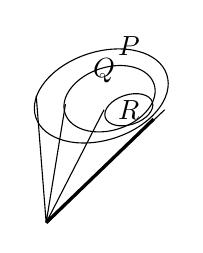
\begin{tikzpicture}[x=.7cm,y=.7cm]
\coordinate (v) at (0,0);
\draw[rotate around={18:(1,2.3)}] (1,2.3) ellipse (1.25 and .8);
\draw[rotate around={18:(1.15,2.25)}] (1.15,2.25) ellipse (.85 and .57);
\draw[rotate around={18:(1.5,2.05)}] (1.5,2.05) ellipse (.45 and .27);
\draw (v)--(-.18,2.3) (v)--(.35,2.15) (v)--(1.05,2.05) (v)--(2.15,2.05);
\draw[very thick] (v)--(1.95,1.88);
\node at (1.5,3.2) {$P$};\node at (1.05,2.75) {$Q$};\node at (1.5,2.05) {$R$};
\end{tikzpicture}}
\[\overline R\subset\unsure{\overline P^{\,0}|P^0}\cap Q=P^0=\overline P^{\,0},\quad\deleted{\unsure{a}}\quad\text{d'où}\]
\deleted{$\boxed{\unsure{\overline R\subset R}}\quad\unsure{\text{donc }P^0}$}
\[R=\mathring{\overline R}\subset\mathring{\overline{P^0}},\quad\text{je dis qu'on a \uline{égalité}, car}\]
\[\mathring{P^0}\subset\mathring Q\quad\text{et on applique le critère de Nakai}\]
\diagram{\boxed{\begin{array}{ccc|c}
R=\mathring{\overline R}&=&\mathring{P^0}\subset&\mathring Q\\
\overline R=P^0&=&\overline P^{\,0}\subset&Q
\end{array}}}

\uline{Question}\quad $xP>0\ \overset{?}{\Longrightarrow}\ x\in R$

Par Nakai, il reste à voir si $\uline{x^2>0}$

\deleted{Donc} $x^2\geq0$, il reste à voir $x^2\neq0$

On peut supposer que $x$ provient de $D$ div. tel que $D^2=0$. Mais alors $\chi(\mathcal L(nD))=\chi(X)+n\chi(D)$ et $h^0(\mathcal L(nD))\geq\chi(\mathcal L(nD))$ pour $n$ grand par Mumford, on doit donc avoir $\chi(D)\unsure{<|\leq}0$
\margin{95}
\scanpage{97}
Soit $u'$ le composé $\deleted{\unsure{u'_{j,n}}}\quad B\quad E_{k,n}\qquad E'_{j,n}\ {\vphantom{E'}}^{u'_{j,\unsure{n|h}}}\ D'$, où la première flèche est l'hom de transition, alors $u'$ est le relèvement cherché.

Mettre le corollaire 2.2. sous forme de l'équivalence de trois conditions (i) $B$ form simple (ii) Condition $1^\circ$ et $2^\circ$ (iii) $\widehat B$ est isomorphe comme alg top à $\widehat {B'}$, où $B'$ est l'algèbre symétrique d'un $C$-module projectif, munie de \unsure{sa|la} topologie définie par son idéal d'augmentation. La forme (iii) est en effet parfois commode, et est obtenue directement dans la démonstration.
\margin{\figure{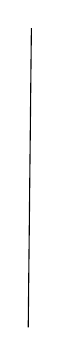
\begin{tikzpicture}\draw (0,0)--(-.04,-3.8);\end{tikzpicture}}}
\margin{\unsure{(i bis)} Pour tout hom de $B$ dans \deleted{une \unsure{$A$-algèbre, quotient} $\unsure{C'|B'}\ D'/J$}, $B'$ \deleted{\unsure{discrète et}} considérée comme quotient d'un \unsure{$\Lambda_D$|$A_D$}. \unsure{polynômiale tronquée}, \deleted{\unsure{on peut relever}} \unsure{on a un} \deleted{$C[t]$} $B'_{\unsure{(i)|i}}$ de $B'_0=C$, \unsure{on peut relever}}
\margin{$\unsure{B'I/I^2}\ \longleftrightarrow$\quad de type fini}

Dans la suite du paragraphe Cohen, 3.4. devient un corollaire immédiat de 3.3. grâce à 2.2. D'ailleurs 3.3. admet toute une kyrielle de corollaires qui dans ma rédaction étaient dans un ordre assez chaotique, je suggère \deleted{\unsure{le}} l'ordre suivant:

$1^\circ$ Existence d'un corps de représentants dans un anneau \inserted{local noeth} complet, quand l'extension résiduelle est séparable. (Cf 3.5.)

$2^\circ$ (oublié dans ma rédaction). Soit $A$ anneau local noeth complet. Les conditions suivantes sont équivalentes: (i) $A$ contient un corps

(ii) Si $\operatorname{car}k(A)=p\quad0$, alors $pA=0$ (iii) $A$ est isomorphe à un anneau quotient d'un anneau $k\ T_1,\ldots,T_n$ sur un corps $k$. (iv) (Si $A$ est intègre de corps des fractions $K$) $k(A)$ et $K$ ont même caractéristique. On peut se borner à donner (iv) à titre de commentaire (c'est une autre façon d'énoncer (ii) simplement), pour \deleted{\unsure{rappeler}} rappeler l'ancienne terminologie ``cas d'égale caractéristique''. Je suggère que nous ne suivions pas cette terminologie, car il est aussi court de dire ``$A$ contient un corps'', et la terminologie ``égale car'' est fort ambigue pour des anneaux non intègres, par exemple artiniens.
\margin{96}
\scanpage{98}
\[H^2\left(L^{\otimes\unsure{n|m}}\otimes K^{\otimes(2\unsure{n|m}-1)}\right)\]
\hrulefill
\diagram{\begin{tikzcd}[ampersand replacement=\&,row sep=large,column sep=small]
\deleted{D^d}\&\boxed{\begin{cases}D^d>0\\D^{\deleted{\unsure{n}}}.C>0\quad\text{si }C>0\end{cases}}\arrow[d,Leftrightarrow,start anchor=west,end anchor=west]\\
\&\boxed{\underbrace{D\in P_1^{+0}},\quad\alpha_{d-1}D^{d-1}\in P_1^+}\arrow[dr,Rightarrow,"{\substack{\text{hyp de}\\\text{réc}}}"',start anchor=south west]\\
\&\&\deleted{\unsure{\alpha(}}D^{d-1}\deleted{\unsure{)}}\in P_{d-1}^{+0}
\end{tikzcd}}

\uline{Question}\quad $\alpha_{d-1}(P_{d-1}^{+0})\subset P_1^+$

\diagram{\fbox{\begin{tikzcd}[ampersand replacement=\&,column sep=large,row sep=large]
P_i^{+0}\subset A^i\arrow[r,"\alpha_i"]\arrow[d,equal,start anchor=south west,end anchor=north west]\&A_{\deleted{\unsure{2}}d-i}\supset P_{\deleted{\unsure{2}}d-i}^+\\
P_+^0\&\\
P_{\deleted{\unsure{2}}d-i}^{+0}\subset A^{2d-i}\arrow[r,"\alpha_{d-i}"]\&A_i\supset P_i^+\\
\operatorname{int}(P_i^{+0})\arrow[r]\&P_{\deleted{\unsure{2}}d-i}^+
\end{tikzcd}}}

\[\unsure{c_i(E)}\]
\margin{97}
\scanpage{99}
$0_{\mathrm{IV}}$\quad\uline{Différentielles et dérivations.}

\deleted{NB} Il nous a paru utile de développer les notions différentielles en utilisant la notion d'algèbre topologique formellement simple,définie dans ``Cohen''. Dans les premiers numéros qui suivent, nous n'utiliserons que la définition ``Cohen''1.1. et éventuellement une partie des sorites contenus dans 1.2.

NB Il se trouvera donc que cette rédaction contient un bon nombre de résultats de ma rédaction ``Cohen différentiel'', qu'il y aura lieu de refondre en conséquence.

1. \uline{Dérivations et extensions d'algèbres}.

\uline{Proposition} 1.1. Soient $A$ un anneau, $B$ une $A$-algèbre, $p:E\quad C$ un homomorphisme de $A$-algèbres dont le noyau $J$ est de carré nul, $u:B\quad C$ un homomorphisme de $A$-algèbres. Supposons qu'on ait un homomorphisme de $A$-algèbres $v_1:A\quad E$ qui relève $u$ i.e. tel que $pv_1=u$. Pour qu'une application $v_2:B\quad E$ ait la même propriété, il f et s qu'on ait
\[v_2-v_1=D\quad\text{i.e.}\quad v_2=v_1+D\]
\margin{$\unsure{\supset}$}
où $D:B\quad J$ est un application satisfaisant les deux conditions suivantes: $1^\circ$ $D$ est $A$-linéaire $2^\circ$ pour $f,g\quad B$, on a $D(fg)=fDg+D(f)g$
\margin{$\unsure{\supset}$}

On notera que compte tenu de $2^\circ$), $1^\circ$) équivaut aussi à \deleted{1 bis}

1 bis) $D$ s'annule sur $\operatorname{Im}(A\quad B)$.

\uline{Définition} 1.2. D'une dérivation d'un anneau dans un module, d'une $A$-dérivation d'une $A$-algèbre $B$ dans un $B$-module $J$.

\uline{Corollaire} 1.3. Etant donnés $A,B$, \deleted{$E$} $p:E\quad C,J$, $u:B\quad C$ comme dans 1.1. \deleted{\unsure{Etant ainsi} pour tout relèvement} l'ensemble des relèvements de $u$ en un homomorphisme $v$ de $A$-algèbres est vide, ou un ensemble principal homogène sous l'action du groupe $\operatorname{Dér}_A(B,J)$
\margin{98}
\scanpage{100}
\diagram{\begin{tikzcd}[ampersand replacement=\&,row sep=large]
D^{\unsure{1}}.C\geq0\quad\text{si}\quad C>0\arrow[d,Rightarrow,"?"]\\
D^iX_i\geq0\quad\text{si}\quad X_i>0\quad??
\end{tikzcd}}

\[D^{\unsure{1}}\in P_1^{+0}\quad\Longrightarrow\quad D^i\in P_i^{+0}\quad\text{pour }i\leq d-1\]
\margin{\uline{hyp. de réc.}}
\deleted{$\unsure{D^2}$}\quad aura-t-on\quad $D^d\in P_d^{+0}$\quad i.e.\quad $D^d\geq0\quad??$

On a
\diagram{\begin{array}{ccccc}
D^d=&D^i&D^{d-i}&& (0<i<d)\\
&\rotatebox{90}{$\ni$}&\rotatebox{90}{$\ni$}\\
&P_i^{+0}&P_{d-i}^{+0}
\end{array}}

\diagram{\begin{tikzcd}[ampersand replacement=\&,row sep=large,column sep=large]
\boxed{P_i^{+0}.P_{d-i}^{+0}\geq0\quad?}\arrow[d,Leftrightarrow,start anchor=east,end anchor=east]\&P_i^{+0}P_j^{+0}\subset P_{i\unsure{+|\cdot}j}^{+0}\arrow[l,Rightarrow]\\
\boxed{\alpha_i(P_i^{+0})\subset P_{d-i}^+}\arrow[d,no head,to path={-- ++(.12,-.3) .. controls +(0,-.3) and +(0,.3) .. (\tikztotarget) \tikztonodes}]\&\\
\boxed{\alpha_{d-i}(P_{d-i}^{+0})\subset P_i^+}\&
\end{tikzcd}}

\[D.C\geq0\quad\text{si }C\geq0\]
\diagram{\begin{tikzcd}[ampersand replacement=\&]
D^2.\deleted{\unsure{D}}D'\geq0\quad\text{si }D'\geq0\arrow[d,Rightarrow,"?"]\\
D^3\geq0
\end{tikzcd}}
\figure{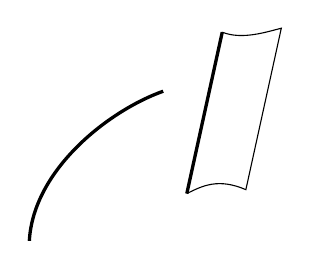
\begin{tikzpicture}[x=1cm,y=1cm]
\draw[very thick] (0,0) .. controls (.05,.9) and (1,1.65) .. (1.7,1.9);
\draw[very thick] (2,0.6)--(2.45,2.65);
\draw (2.45,2.65) .. controls (2.7,2.55) and (3,2.65) .. (3.2,2.7)--(2.75,.65) .. controls (2.4,.8) and (2.2,.7) .. (2,.6);
\end{tikzpicture}}

\diagram{\begin{tikzcd}[ampersand replacement=\&]
P_1^{+0}\subset A^1\arrow[r]\&A_2\supset P_2^+
\end{tikzcd}}
\deleted{$\unsure{D}+{}$}\quad $D'+nD\in P_2^+$
\[\begin{aligned}
(D'+nD)^3={}&D^{\unsure{\prime|!}3}+3nD'^2D\\
&+3n^2D'D^2+n^3D^3
\end{aligned}\]
\figure{\begin{tikzpicture}[x=1cm,y=1cm]
\draw (2.7,1.4) .. controls (3,1.6) and (3.3,1.7) .. (3.5,1.7);
\draw (0,0) .. controls (.05,.35) and (.4,.75) .. (.65,.9);
\draw (1.5,-.05) .. controls (1.9,.1) and (2,.3) .. (2.05,.5);
\draw[very thick] (3,.15) .. controls (3.35,.35) and (3.55,.6) .. (3.65,.9);
\node[draw,below] at (1.9,-.2) {$D^3\geq0$};
\end{tikzpicture}}
\figure{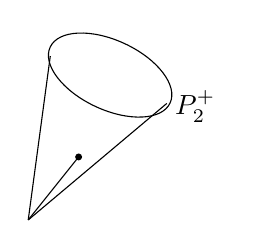
\begin{tikzpicture}[x=.8cm,y=.8cm]
\draw[rotate around={-25:(1.3,2.3)}] (1.3,2.3) ellipse (1.05 and .55);
\draw (0,0)--(.35,2.6) (0,0)--(2.2,1.85);
\draw (0,0)--(.8,1);\fill (.8,1) circle (.055);
\node at (2.65,1.8) {$P_2^+$};
\end{tikzpicture}}
\deleted{$\unsure{D+\frac1n D'}$}
\[D'+nD\simeq\]
\margin{99}
\scanpage{101}
\mspage{\unsure{95|45}}
\diagram{\begin{tikzcd}[ampersand replacement=\&,row sep=large,column sep=large]
E'_{j,n}\arrow[r,no head,"\unsure{v_i|u_i}"]\&E^{\deleted{\prime}}_{i,n}\\
E'_{k,n}\arrow[u]\arrow[r,no head,"\unsure{v_j|u_j}"]\&E_{j,n}\arrow[u]
\end{tikzcd}}
où les flèches verticales sont les homomorphismes de transition.

N.B. On pose $E_{i,n}=E_i/I_i^{n+1}$, $E'_{i,n}=\operatorname{Symm}_{C_i}(I_i/I_i^2)/$ puissance $(N+1)$ème de l'\unsure{idéan|idéal} d'augmentation. La démonstration de lemme B est immédiate, en procédant comme dans le cas particulier 2.2. déjà traité.

\uline{Lemme} C Supposons $C$ et $B$ form simple sur $A$, (donc en vertu de lemme A les conditions de Lemme B sont vérifiées). Alors:

\inserted{a)} Pour tout \deleted{$i$, \unsure{existe un} $j\unsure{>|,}i$ et un $v_i$ comme dans lemme B a), avec en plus un} système $i,j,v_i$ comme dans Lemme B\inserted{a)}, \deleted{il existe un}\inserted{il existe} $k\geq j$ \inserted{et}\deleted{\unsure{qui soit} rendant valable la conclusion de lemme B, b), et tel qu'il existe} un homomorphisme de $A$-algèbres $w_j:E_{k,n}\mathbin{-}E'_{j,n}$ ayant les propriétés suivantes: $1^\circ$) \inserted{$w_{\unsure{n|k}}$} induit un épimorphisme sur les gradués associés $2^\circ$) $v_iw_j$ est l'homomorphisme de transition $E_k\to E_{\unsure{i}}$

\deleted{b) Soient $i,j,k,v_i,v_j,w_j$ comme dans a). Alors il existe un $\unsure{\ell}\quad k$, un homomorphisme $v_k:E'_{\unsure{\ell|k},n}\quad E_{k,n}$ et un homomorphisme $w_k:E_{\unsure{\ell|k},n}\ \deleted{\unsure{E}}\ E'_{k,n}$ ayant les propriétés suivantes: $1^\circ$) $v_k$ a les propriétés mentionnées déjà pour $v_i,v_j$ $2^\circ$) $w_k$ a les deux propriétés mentionnées déjà pour $w_j$ $3^\circ$}
\margin{100}
\scanpage{102}
conjectures de

Lefschetz pour

cycles Algébriques:

\diagram{\left\{\begin{array}{l}
\text{Extension aux \uline{Jac.\unsure{inter.|intr.}}}\\
\text{Conjectures \uline{locales}}
\end{array}\right.}
\margin{101}
\scanpage{103}
$X$ surface projective non sing.

$Y$ section hyperplane non sing.

\diagram{\begin{tikzcd}[ampersand replacement=\&]
\unsure{N^1}(X)\arrow[r]\&\unsure{N^1}(Y)
\end{tikzcd}}
surjectif mod grp fini\quad noyau de rang $\unsure{\rho\,1|\rho-1}$

\diagram{\begin{tikzcd}[ampersand replacement=\&]J^1(X)\arrow[r]\&J^1(Y)\end{tikzcd}}
injectif exc. $p$

\diagram{\begin{tikzcd}[ampersand replacement=\&]A^1(X)\arrow[r]\&A^1(Y)\end{tikzcd}}
noyau $K$ tel que $K\cap J^1(X)$ fini,
\uline{donc} $K$ de type fini

Soit $B^1(X)$, ``partie primitive'' de $\unsure{A^1}(X)$, \unsure{formée} des classes de div. de \uline{degré} $0$, donc
\diagram{\begin{tikzcd}[ampersand replacement=\&]B^1(X)\arrow[r]\&J^1(Y)\end{tikzcd}}
$[\ B^1(X)$ contient $K\ ]$

\diagram{\begin{tikzcd}[ampersand replacement=\&,column sep=large]
\deleted{\unsure{0\to}}\&K\arrow[r,"{\substack{\text{inj.}\\\text{mod grp}\\\text{fini}}}"']\&\unsure{M^1|N^1}(X)\arrow[r]\&\underbrace{J^1(Y)/\operatorname{Im}J^1(X)}_{\substack{\text{partie ``mobile''}\\\text{de }J^1(Y)}}
\end{tikzcd}}

\deleted{\uline{Question} Une classe de $\unsure{M^1|N^1}(X)$ dont l'image dans $J^1(Y)/J^1(X)$ \unsure{est} nulle, est-elle dans $K$ \inserted{i.e. dans $\operatorname{Im}K$}}

N.B. ``En général'' $\unsure{M^1|N^1}(X)\to J^1(Y)/J^1(X)$ est injectif mod grp finis, donc $K$ fini

Je présume qu'il en est ainsi si les \unsure{positions} limites de $Y$ dans les pinceaux \unsure{plans} contenant $Y$ sont des courbes \uuline{irréductibles}...
\margin{102}
\scanpage{104}
\mspage{- 115 -}
toute sous-algèbre de type fini de $C\inserted{[}T\inserted{]}$ vérifie la condition des chaînes, il en est de même de toute sous-algèbre de type fini de $C_{\uline{\unsure{r|p}}}\inserted{[}T\inserted{]}$, ce qui achève la démonstration.

\margin{$\boxed{\begin{gathered}\dim\uline O_x\leq\dim\uline O_y+\dim(\unsure{\uline O_x\otimes k(y)})-\delta(x)\\
\delta(x)=\deleted{\unsure{\deg}}\inserted{\dim_{\unsure{x}}}f^{-1}f(x)-e\end{gathered}}$}

\uline{Corollaire 1 .- Soient $Y$ un préschéma irréductible localement noethérien}, $X$ \uline{un préschéma irréductible}, $f:X\inserted{\to}Y$ \uline{un morphisme} \deleted{\illegible{1}} \uline{dominant de type fini. Soit} $\inserted{\xi}$ (resp.\ $\inserted{\eta}$) \uline{le point générique de} $X$ (resp. $Y$) \deleted{\unsure{et}}, \uline{et soit} $e=\dim(f^{-1}(\inserted{\eta}))=\deg.\operatorname{tr}_{\inserted{\uline{\kappa}(\eta)}}\inserted{\uline{\kappa}(\xi)}$ (``dimension de la fibre générique)''). \uline{Pour tout} $x\inserted{\in}X$, \uline{on a, en posant} $y=f(x)$
\[
(13)\qquad e+\operatorname{codim}_Y\overline{\inserted{\{}y\inserted{\}}}\inserted{\geq}\deg.\operatorname{tr}_{\inserted{\uline{\kappa}(y)}}\inserted{\uline{\kappa}(x)}+\operatorname{codim}_X\overline{\inserted{\{}x\inserted{\}}}.
\]
\margin{formule hybride, donner plutôt \uline{deux} formules l'une en termes d'alg. comm., l'autre en termes ``géom.''}

\uline{En outre, les deux membres sont égaux lorsque} $\uline{O}_y$ \uline{est un quotient d'anneau local régulier}.
\margin{\deleted{\unsure{si}} cond. des chaînes \unsure{stricte}}
\margin{\uuline{Variante}\quad\uuline{en vue}\quad$\left\{\begin{gathered}\dim\uline O_x\leq\dim\uline O_y+\dim\uline O_x\otimes k(\unsure{y|x})\\
-[\dim_xf^{-1}f(x)-\unsure{e}]\end{gathered}\right.$}

Comme la question est locale, on peut supposer $X$ et $Y$ affines\inserted{(et réduits)}. \deleted{\unsure{En effet} \illegible{15} \unsure{pour} \illegible{8}}\inserted{soient} $X=\operatorname{Spec}(B)$, $Y=\operatorname{Spec}(A)$, où $B$ est une algèbre intègre de type fini sur $A$; comme $f$ est dominant, $A$ s'identifie à une sous-algèbre de $B$ (§ 1,n°2,cor.4 de la prop.5), donc $\uline{O}_y$ à une sous-algèbre de $\uline{O}_x$. Comme $\inserted{\uline{\kappa}(\eta)}$ et $\inserted{\uline{\kappa}(\xi)}$ sont les corps de fractions de $A$ et $B$ respectivement, donc de \deleted{$O_x$} $\uline{O}_y$ et $\uline{O}_x$ respectivement, la formule (13) résulte de (12) appliquée aux anneaux $\uline{O}_y$ et $\uline{O}_x$.
\margin{\deleted{Si $\unsure{Z}\subset X$ fermé irréductible, alors $\dim_{\unsure{x}}f^{-1}f(x)$} \unsure{n'énoncer} \illegible{3}}
\margin{\figure{\begin{tikzpicture}\draw[->] (2,2)--(0,0);\end{tikzpicture}}}

On notera d'ailleurs que $\deg.\operatorname{tr}_{\inserted{\uline{\kappa}(y)}}\inserted{\uline{\kappa}(x)}$ n'est autre que la dimension de $f^{-1}(y)\inserted{\cap}\overline{\inserted{\{}x\inserted{\}}}$, comme il résulte de la prop.7 du n°2, appliquée à $f^{-1}(y)$ considéré comme préschéma algébrique sur $\inserted{\uline{\kappa}(y)}$. En particulier:
\margin{\deleted{\unsure{dim}}}

\uline{Corollaire 2} .- \deleted{\unsure{Si}} \uline{Les hypothèses du cor.1 étant vérifiées, supposons en outre que $x$ soit fermé dans $f^{-1}(y)$ et que $\uline{O}_y$ soit un quotient d'anneau régulier. Alors}
\margin{\deleted{\unsure{si}} cond. des chaînes \unsure{stricte}}
\[
(14)\qquad\operatorname{codim}_X\overline{\inserted{\{}x\inserted{\}}}=e+\operatorname{codim}_Y\overline{\inserted{\{}y\inserted{\}}}.
\]
\uline{Corollaire 3 .- Les hypothèses du cor.1 étant vérifiées, on a}
\margin{103}
\scanpage{106}
\uline{Conjectures ``Lefschetz'' locales}

\(S=\operatorname{Spec} A,\quad A\) anneau str. local noeth,
\[
f\in\unsure{\mathfrak r A|\operatorname{rad}A},\qquad
\left\{\begin{array}{l}X=S-\text{pt fermé}\\Y=X\cap V(f)\end{array}\right.
\]
\(X,Y\) réguliers
\[
U=X-Y
\]

\textcircled{1}
\[
\begin{array}{lll}
\deleted{\unsure{2}}i\unsure{\geq|=}\dfrac N2&
N_{\unsure{\ell}}^i(X)\equiv\deleted{\text{fini}}0&\text{(mod grp finis)}\\[4pt]
i\geq\dfrac{N+1}{2}&N^i(X)\deleted{\unsure{\neq|\equiv}}\equiv0&\text{(mod grp finis)}\\
&J^i(X)\equiv0&\\[4pt]
&\text{i.e. }A^i(X)\equiv0&\text{(mod grp finis)}
\end{array}
\]

\textcircled{2}
\diagram{\begin{array}{lll}
J^i(X)\ \unsure{\longrightarrow|\text{---}}\ J^i(Y)&
\text{bij. }\inserted{\text{exc. }p}\text{ si }i\leq\dfrac{N-2}{2}\\
&\text{inj }\inserted{\text{exc. }p}\text{ si }i\leq\dfrac{N-1}{2}\\
&\text{nul si }i\geq\dfrac N2
\end{array}}
\margin{[N.B. Si \(i\geq\dfrac N2\), \(J^i(Y)=0\) ! d'ailleurs si \(i\geq\dfrac{N+1}{2}\) on a \(J^i(X)=J^i(Y)=0\)]}
\margin{Cas critique \(J^{\frac{N-1}{2}}\quad J^{\frac N2}\)
\figure{
\begin{tikzpicture}[x=.6cm,y=.6cm]
\draw[line width=2.4pt] (0,.3)--(0,0)--(.8,-.1)--(.8,.35);
\draw (0,.19)--(.8,-.02);
\end{tikzpicture}}}

\diagram{\begin{array}{ll}
N^i(X)\ \unsure{\longrightarrow|\text{---}}\ N^i(Y)&
\text{bij }\inserted{\text{\tikz[baseline=(n.base)]\node[draw,ellipse,inner sep=1pt](n){exc. \(p\)};}}\text{ si }i\leq\dfrac{N-3}{2}\\
&\text{inj }\inserted{\text{\tikz[baseline=(n.base)]\node[draw,ellipse,inner sep=1pt](n){exc. \(p\)};}}\text{ si }i\leq\dfrac{N-2}{2}\\
&\text{nul }\inserted{\text{\tikz[baseline=(n.base)]\node[draw,ellipse,inner sep=1pt](n){mod. grp finis};}}\text{ si }i\geq\dfrac{N-1}{2}
\end{array}}
\margin{[N.B. si \(i\geq\dfrac{N-1}{2}\), on a \(N^i(Y)\equiv0\); si \(i\geq\dfrac N2\), on a \(N^i(X)=N^i(Y)\equiv0\) \unsure{etc.}]}
\margin{105}
\scanpage{107}
\margin{Cas critique \(N^{\frac{N-2}{2}},\ N^{\frac{N-1}{2}}\)
\figure{
\begin{tikzpicture}[x=.5cm,y=.5cm]\draw[line width=1.2pt](0,.3)--(0,0)--(1,0)--(1,.3);\end{tikzpicture}}}

\diagram{\begin{array}{ll}
A^i(X)\ \unsure{\text{---}|\longrightarrow}\ A^i(Y)&\text{bij si }i\leq\dfrac{N-3}{2}\\
&\text{inj. si }i\leq\dfrac{N-2}{2}
\end{array}}
\margin{Cas critiques \(i=\dfrac{N-2}{2},\ \dfrac{N-1}{2},\ \dfrac N2\)}

\margin{\unsure{conséquence} de 1° et 2°}
\textcircled{3}
\diagram{\begin{array}{ll}
A^i(X)\longrightarrow A^i(U)&\text{\uline{un isom} mod grp finis, }\forall i\\
&\text{\uline{un} \uline{isom} si }i\leq\dfrac{N-1}{2}
\end{array}}
\margin{[N.B. si \deleted{\(\unsure{i\geq N}\)} \(i\geq\dfrac{N+1}{2}\), \(A^i(X)\) et \(A^i(U)\) sont finis !]}
\diagram{\begin{array}{ll}
A^i(Y)\longrightarrow A^{i+1}(X)&\text{\uline{nul} \unsure{mod} grp finis, }\forall i\\
&\text{nul si }i\leq\dfrac{N-1}{2}
\end{array}}
\margin{[N.B. si \(i\geq\dfrac N2\), \(A^i(Y)\) est un grp fini !]}

\textcircled{4}\quad\uline{Pb}\quad Définir des formes ``\unsure{d'intersections|d'intersection}''
\[
N^i(X)\times N^i(X)\ \unsure{\longrightarrow|\text{---}}\ Z\ ??
\]
Définir pour \(J^{\unsure{\frac{N-1}{2}|\frac{N-2}{2}}}(X)\longrightarrow J^{\frac{N-1}{2}}(Y)\) resp. \(N^{\frac{N-2}{2}}(X)\longrightarrow N^{\frac{N-1}{2}}(Y)\) une théorie des cycles évanescents \(\text{------}\)
\figure{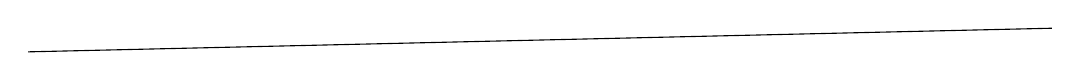
\begin{tikzpicture}\draw (0,0)--(13,.3);\end{tikzpicture}}

\uline{Ex}\quad \(N=2\)

\textcircled{1}\quad\(\boxed{N^1(X)\ \text{fini}}\) : c'est le th. \uline{de \deleted{\unsure{Lef}} Mumford-Hodge}.

\textcircled{2}\quad vide

\textcircled{3}\quad \deleted{\(\unsure{A^1(X)}\longrightarrow\)} vide

Groupe \(\unsure{+}\) essentiel \(J^1(X)\)
\margin{106}
\scanpage{108}
\uline{Ex}\quad \(N=3\)

\textcircled{1}\quad \(\boxed{A^2(X)\ \text{fini}}\) en particulier \(J^2(X)=0\)

\textcircled{2}\quad
\diagram{\begin{array}{|l}\hline J^1(X)\longrightarrow J^1(Y)\quad\text{injectif exc. }p\\\hline\end{array}}
\deleted{\unsure{facteurs}}

\textcircled{3}\quad \deleted{\(\unsure{A^1(X)}\)} contenu dans 1°)

groupes essentiels \(J^1(X),N^1(X)\) définissant \(A^1(X)\)

hom essentiels
\diagram{\begin{array}{ll|l}
J^1(X)\longrightarrow J^1(Y)&&A^1(X)'\longrightarrow J^1(Y)\\
N^1(X)'\longrightarrow J^1(Y)&&
\end{array}}
\margin{\unsure{ssgrp} d'indice fini de \(N^1(X)\)}
\figure{\begin{tikzpicture}\draw(0,0)..controls(.5,.15)and(.75,-.15)..(1,.05);\end{tikzpicture}}

\uline{Pb} définir un complémentaire naturel de \(J^1(X)\) dans \(J^1(Y)\) (\unsure{correspdt.} aux ``cycles évanescents'')

Donner un sens à la formule
\[
J^1(X)\xrightarrow{\sim}J^1(Y)^\pi
\]
Interpréter le th. de \inserted{l'index de} Hodge pour les surfaces projectives en termes de la négativité d'une certaine forme définie sur \(N^1(X)\)\ldots ?

\uline{Ex}\quad \(N=4\)

\textcircled{1}\quad
\[
\left\{\begin{array}{l}N^2(X)\ \text{fini}\\A^3(X)\ \text{fini, en particulier }J^3(X)=0\end{array}\right.
\]
\textcircled{2}\quad
\diagram{\begin{array}{ll}
J^1(X)\longrightarrow J^1(Y)&\text{bij exc. }p\\
\deleted{J}N^1(X)\longrightarrow N^1(Y)&\text{inj. exc. }p\\
\Rightarrow\ A^1(X)\longrightarrow A^1(Y)&\text{\uline{bij exc.} }p
\end{array}}
\textcircled{\unsure{3}}
\margin{107}
\scanpage{109}
groupes essentiels \(J^2(X),N^1(X)\)

hom essentiel
\diagram{\begin{array}{ccc}N^1(X)&\unsure{\text{---}|\longrightarrow}&N^1(Y)\end{array}}

\uline{Pb} définir un complémentaire naturel de \(N^1(X)\) dans \(N^1(Y)\) (cycles évanescents). \deleted{Donner}

Donner un sens à la formule
\[
\deleted{\unsure{J}}N^1(X)\xrightarrow{\sim}N^1(Y)^\pi
\]
\figure{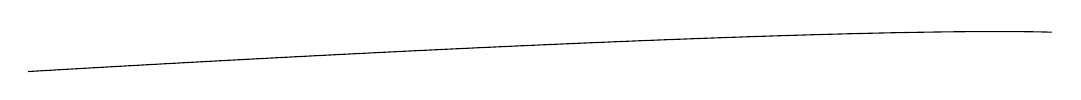
\begin{tikzpicture}\draw(0,0)..controls(6,.35)and(11,.55)..(13,.5);\end{tikzpicture}}

Cas important \(N=2m+1\), à \unsure{prouver} alors
\[
A^{m+1}(X)\equiv0\qquad(\text{et }A^i(X)\equiv0\text{ si }i\geq m+1)
\]
[Cas \(N=2m\), alors \(N^m(X)\equiv0\) i.e. \(J^m(X)\equiv A^m(X)\),

et \(A^{m+1}(X)\equiv0\ \unsure{\sim}\ (\text{et }A^{\deleted{m}\inserted{i}}(X)\equiv0\text{ si }i\geq m+1)\)]
\margin{108}
\scanpage{111}
\uline{Conjectures} \inserted{``\uline{Lefschetz}''}\quad(\(k\) alg. clos)

Soit \(X^n\) projectif lisse connexe, \(Y\) \unsure{une} section hyperplane lisse.
\[
\begin{array}{ll}
-\quad A_r^i(X)\ \cdots&\text{cycles de codimension }i\text{ mod équivalence }\deleted{\text{alg}}\inserted{\text{rationnelle}}\\
A_a^i(X)&\text{algébrique}\\
A_\tau^i(X)&\text{équivalence }\tau
\end{array}
\]

\textcircled{1}\quad
\diagram{\begin{tikzcd}[ampersand replacement=\&]A_r^i(X)\arrow[r]\&A_r^i(Y)\end{tikzcd}}
\deleted{\diagram{\boxed{\begin{array}{llll}
\text{bijectif }\inserted{\text{exc. }p}&\text{si }2i\leq n-2&\text{i.e. }i<\dfrac{n-1}{2}\\
\text{injectif exc. }p&\text{si }2i\leq n-1&\text{i.e. }i\leq\dfrac{n-1}{2}\\
\text{bijectif }\deleted{\text{exc. }p.}&\unsure{\text{si}}\ \unsure{2i<n}
\end{array}}}}

\(2i\leq n-2\)\quad i.e. \deleted{\unsure{si}} \(i<\dfrac{n-1}{2}\)

bijectif [exc. \(p\) ?]

\(2i=n-1\)\quad i.e. \(i=\dfrac{n-1}{2}\)

injectif [exc. \(p\),]

induit
\diagram{\begin{array}{ll}
A_r^i(X)^\tau\longrightarrow A_r^i(Y)^\tau&\text{bijectif [exc. }p\text{]}\\
\Rightarrow\ A_a^i(X)\longrightarrow A_a^i(Y)&\text{bijectif [exc. }p\text{]}\\
A_\tau^i(X)\ \unsure{\text{---}|\longrightarrow}\ A_\tau^i(Y)&\text{injectif}
\end{array}}

\(2i=n\deleted{\unsure{+1|+2}}\)\quad i.e. \(i=\dfrac{n\deleted{\unsure{+1|+2}}}{2}\)

induit
\diagram{\begin{array}{ll}A_r^i(X)^\tau\ \unsure{\text{---}|\longrightarrow}\ A_{\unsure{r|a}}^i(Y)^\tau&\text{injectif [exc. }p\text{]}\end{array}}

\textcircled{2}\quad
\diagram{\begin{tikzcd}[ampersand replacement=\&]A_i^r(Y)\arrow[r]\&A_i^r(X)\end{tikzcd}}

\(2i\leq n-3\)\quad i.e. \(i\leq\dfrac{n-3}{2}\deleted{\unsure{=\frac{n-1}{2}+1}}=\dfrac{n-1}{2}-1\)

bijectif [exc. \(p\) ?]

\(2i=n-2\)\quad i.e. \(i=\dfrac{n-2}{2}\)
\diagram{\left\{\begin{array}{lll}
\text{surjectif [exc. }p\text{,]}&&\\
\text{induit}&A_i^r(Y)^\tau\ \unsure{\text{---}|\longrightarrow}\ A_i^r(X)^\tau&\text{surj. [exc. }p\text{]}\\
\text{induit}&A_i^a(Y)\longrightarrow A_i^a(X)&\text{bij. [exc. }p\text{]}
\end{array}\right.}
\margin{110}
\scanpage{112}
\(2i=n-1\)\quad i.e. \(i=\dfrac{n-1}{2}\)

induit
\diagram{\begin{array}{ll}A_i^\tau(Y)\ \unsure{\text{---}|\longrightarrow}\ A_i^\tau(X)&\text{surj. exc. }p\end{array}}

\textcircled{3}\quad
\diagram{\begin{tikzcd}[ampersand replacement=\&]A_a^i(X)\arrow[r,"E^{n-2i}"]\&A_a^{n-i}(X)\end{tikzcd}}
\((2i\leq n)\)

\deleted{injectif exc. \(p\)}\inserted{bijectif} mod groupes finis

\deleted{induit \diagram{\begin{array}{ll}A_\tau^i(X)\ \unsure{\text{---}|\longrightarrow}\ A_\tau^{n-i}(X)&\text{bijectif mod groupes finis}\end{array}}}

\diagram{\begin{tikzcd}[ampersand replacement=\&]A_{\deleted{\unsure{\tau|a}}\inserted{r}}^i(X)^\tau\arrow[r,"E^{n-2i+1}"]\&A_r^{n-i+1}(X)^\tau\end{tikzcd}}
\(2i-1\leq n\)

bijectif mod groupes finis

\(\Longrightarrow\)\quad
\diagram{\begin{tikzcd}[ampersand replacement=\&]A_r^i(X)\arrow[r,"E^p"]\&A_r^{i+p}(X)\end{tikzcd}}

a) injectif mod grp finis si \(\unsure{p|r}\leq n-2i\)

b) surjectif mod grp finis si \(p\geq n-2i+1\)
\figure{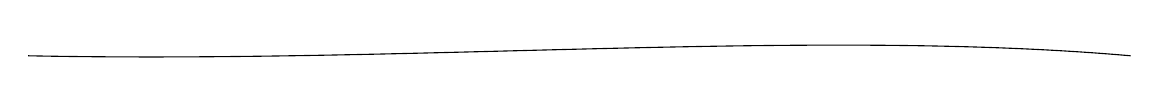
\begin{tikzpicture}\draw(0,0)..controls(5,-.1)and(10,.35)..(14,0);\end{tikzpicture}}
\margin{111}
\scanpage{113}
\textcircled{2'}\quad Posons \(U=X-Y\), qui est une variété affine non sing.
\[
A_r^i(U)\simeq A_r^i(X)/\operatorname{Im}A_r^i(Y),\quad\text{de même pour }A_a^i(U)\ldots
\]
\[
\begin{array}{llll}
2i\leq n-2&\text{i.e. }i\leq\dfrac n2-1&A_i^r(U)\unsure{=|\equiv}0&\text{(exc. }p\text{ ?)}\deleted{\unsure{?}}\\
2i=n-1&\text{i.e. }i=\dfrac{n-1}{2}\deleted{\unsure{+1}}&A_i^a(U)=0&\text{(exc }p\text{ ?)}
\end{array}
\]

\textcircled{3'}\quad Soit \(E\) le cône projectant affine épointé de \(X\), (variété quasi-affine non sing. de dim \(2n+1\)).
\[
\begin{array}{lll}
2i\geq n+2&\text{i.e. }i\geq\dfrac n2+1&A_r^i(E)\ \deleted{\unsure{est}}\text{ fini},\quad A_r^i(E)^a=0\\
&n-i\leq\dfrac n2-1&\\[4pt]
2i\geq n+1&\text{i.e. }i\geq\dfrac{n+1}{2}&A_a^i(E)\ \text{fini}\\
&\text{i.e. }n-i\leq\dfrac{n-1}{2}&
\end{array}
\]

\uline{N.B.} On doit avoir
\[
\left\{\begin{array}{lll}
A_a^i(E)\simeq\deleted{\unsure{B_a^i(X)}}\inserted{\unsure{M_a^i(X)|N_a^i(X)}}&\inserted{\text{\tikz[baseline=(n.base)]\node[draw,ellipse,inner sep=1pt](n){mod groupes finis};}}&\text{si }2i\leq n\\
\deleted{A_{\unsure{r|\tau}}^i(E)^a\simeq B_\tau^i(X)}&\deleted{\text{mod grp finis}}&\deleted{\text{si }2i\leq n\unsure{+1}}\\
A_a^i(E)\simeq0&\text{mod grp finis}&\text{si }2i\geq n+1
\end{array}\right.
\]
\[
\left\{\begin{array}{lll}
A_r^i(E)^a\simeq\inserted{I^i}\deleted{\unsure{B_\tau^i}}(X)&\text{mod grp finis}&\text{si }2i\leq n+1\\
A_r^i(E)^{\unsure{a}}\simeq\unsure{0}&\text{``}&\text{si }2i\geq n+2
\end{array}\right.
\]

où
\[
\unsure{M_a^i|N_a^i}(X)=\operatorname{Ker}\bigl(A_a^i(X)\xrightarrow{L^{n-2i}}A_{\unsure{a}}^{n-i}(X)\bigr)
\]
\margin{partie ``primitive'' de la ``\unsure{ch.|cl.} algébrique''}
\[
\unsure{I^i|I_r^i}(X)=\operatorname{Ker}\bigl(A_r^i(X)^a\xrightarrow{L^{n-2i+1}}A_r^{n-i+1}(X)^a
\]
\margin{partie ``primitive'' de la \unsure{VAb.|V.A.} intermédiaire}
\margin{112}
\scanpage{114}
\deleted{
\uline{Rq}\quad Soit \(A\) un anneau local noeth complet tel que les composantes irréductibles de \(S=\operatorname{Spec} A\) sont ``d'égale dim''. Soit \(f\in\unsure{\mathfrak r A}\), et \(U=S_f\). Alors \deleted{\unsure{pour} \(H^{\unsure{i}}\) \unsure{si}} \(\operatorname{cd}U\leq\dim A\).

On peut supposer \(A\) intègre \inserted{normal,} complet \inserted{de dim \(n\),} et on est ramené à prouver que \(H^i(U,Z/\ell Z)=0\) si \(i>n\).
\(A\) est fini sur un anneau de séries formelles \(A_0=k[[t_1,\ldots,t_n]]\), et on peut supposer d'ailleurs \(K/K_0\) \uline{séparable} (quitte à remplacer \(A\) par la \unsure{normalisé|normalisée} de \(A_0\) dans la clôture sép. de \(K_0\) dans \(K\)\ldots).
\margin{Soit \(\delta\in\unsure{\mathfrak r A_0}\) tel que \(S_\delta\) étale sur \(S_{0\delta}\).}

On \deleted{peut d'ailleurs} \deleted{\unsure{que}} peut supposer \(\delta f=t_n\) [par la \unsure{dém.} du \unsure{th.|R.} de Cohen\ldots]. Posons \(A'_0=\operatorname{Spec} k[[t_1,\ldots,t_{n-1}]]\{t_n\}\), \(S'_0=\operatorname{Spec} A'_0\), le \unsure{R.E.|R.3.} \deleted{\unsure{f}} induit par \(S\vert S_{0\delta f}\) étale provient par chgt de base d'un \(\unsure{Z'|S'}\) étale sur \(S'_{0t_n}\) et \unsure{en|on} fait (par raison de normalité)
\[
S\simeq S_0\times_{S'_0}S',\qquad S'\ \inserted{=\operatorname{Spec}A'}\ \text{\unsure{rev.} fini normal de }S.
\]
D'ailleurs \(f\) provient d'un \(f'\in\unsure{\mathfrak r A'}\).

\margin{\diagram{\begin{tikzcd}[ampersand replacement=\&,column sep=small,row sep=small]
S\arrow[d,no head]\&\\
S_0=\operatorname{Spec}k[[t_1,\ldots,t_n]]\arrow[dr]\&\\
\&S'_0=\operatorname{Spec}k[[t_1,\ldots,t_{n-1}]]\{t_n\}
\end{tikzcd}}}
}
\margin{113}
\scanpage{115}
\deleted{1) \(\unsure{\dim X=n=2}\)}

\uline{Ex.}\quad \(n=2\)

\textcircled{1}
\diagram{\begin{array}{lll}
A_r^0(X)\ \unsure{\text{---}|\longrightarrow}\ A_r^0(Y)&\text{bijectif exc }p&\text{OK}\\
A_r^1(X)^\tau\longrightarrow A_r^1(Y)^\tau&\text{injectif exc. }p&\text{OK}
\end{array}}

\textcircled{2}
\diagram{\begin{array}{lll}
A_0^r(Y)\ \unsure{\text{---}|\longrightarrow}\ A_0^r(X)&\text{surjectif exc. }p&\text{OK}\\
A_0^r(Y)^\tau\ \unsure{\text{---}|\longrightarrow}\ A_0^r(X)^\tau&\text{----}&\text{OK}\\
\begin{array}{ccc}A_0^a(Y)&\longrightarrow&A_0^a(X)\\\Vert&&\Vert\\Z&&Z\end{array}&\text{bijectif exc. }p&\text{OK}
\end{array}}
\margin{du moins si équiv. rat. des 0-cycles = équiv. d'Albanese\ldots}

\textcircled{3}
\diagram{\begin{array}{lll}
\left.\begin{array}{ccc}A_a^0(X)&\xrightarrow{E^2}&A_a^2(X)\\\Vert&&\Vert\\Z&&Z\\A_a^1(X)&\overset{E^0=\mathrm{id}}{\unsure{\text{---}|\longrightarrow}}&A_a^1(X)\end{array}\right\}&\text{bijectif mod grp finis}&\text{OK.}\\[6pt]
\left.\begin{array}{ccc}A_r^0(X)^\tau&\longrightarrow&A_{\unsure{a|r}}^2(X)\\\Vert&&\Vert\\0&&0\\A_r^1(X)^\tau&\xrightarrow{\mathrm{id}}&A_r^1(X)^\tau\end{array}\right\}&\text{bij. mod grp finis}&\text{OK.}
\end{array}}

\textcircled{2'}\quad \(A_0^r(U)=0\)
\margin{O.K. si équivalence rationnelle = équiv. d'Albanese}

\uline{Ex.}\quad \(n=3\)

\textcircled{1}
\diagram{\begin{array}{lll}
A_r^0(X)\ \unsure{\text{---}|\longrightarrow}\ A_r^0(Y)&\text{bij. exc. }p&\text{O.K.}\\
A_r^1(X)\ \unsure{\text{---}|\longrightarrow}\ A_r^1(Y)&\text{injectif exc }p.&\text{O.K.}\\
A_r^1(X)^\tau\ \unsure{\text{---}|\longrightarrow}\ A_r^1(Y)^\tau&\text{bijectif exc }p&\text{O.K.}
\end{array}}

\textcircled{2}
\diagram{\begin{array}{lll}
A_0^r(Y)\ \unsure{\text{---}|\longrightarrow}\ A_0^r(X)&\text{bijectif exc. }p&\text{O.K.}\\
A_1^a(Y)\longrightarrow A_1^a(X)&\text{surjectif exc. }p&\textcircled{?}
\end{array}}
\margin{si équiv. rat. = équiv. Alb.}

\textcircled{3}
\diagram{\begin{array}{lll}
\begin{array}{ccc}A_a^0(X)&\overset{E^3}{\unsure{\text{---}|\longrightarrow}}&A_a^3(X)\\\simeq Z&&\simeq Z\end{array}&\text{bijectif mod grp finis}&\text{OK.}\\
A_a^1(X)\overset{E^1}{\unsure{\text{---}|\longrightarrow}}A_a^2(X)&\deleted{\text{\unsure{bijectif|surjectif}}}&\\
&\text{bijectif mod grp finis}&
\end{array}}
\figure{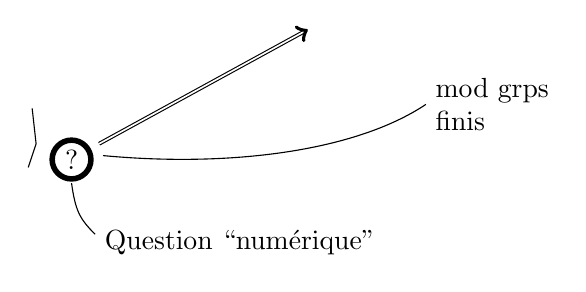
\begin{tikzpicture}[x=1cm,y=1cm]
\node[draw,circle,line width=2pt,inner sep=2pt](q) at(0,0){?};
\draw[->,double] (.35,.2)--(3,1.65);
\draw(0,-.3)..controls(.05,-.65)and(.1,-.75)..(.3,-.95);
\node[anchor=west] at(.3,-1.05){Question ``numérique''};
\draw(.4,.05)..controls(2,-.1)and(3.6,.1)..(4.5,.7);
\node[anchor=west,align=left] at(4.5,.7){\unsure{mod} \unsure{grps}\\finis};
\draw(-.5,.65)--(-.45,.2)--(-.55,-.1);
\end{tikzpicture}}
\margin{114}
\scanpage{116}
\diagram{\begin{array}{lll}
\begin{array}{ccc}A_r^0(X)^\tau&\xrightarrow{E^4}&A_r^{\deleted{\unsure{3}}4}(X)^\tau\\\Vert&&\Vert\\0&&0\end{array}&\text{\unsure{bij exc.} grp finis}&\text{OK}\\
A_r^1(X)^\tau\xrightarrow{E^2}A_r^3(X)^\tau&\text{id}&\text{OK}\\
A_r^2(X)^\tau\overset{\mathrm{id}}{\unsure{\text{---}|\longrightarrow}}A_r^2(X)^\tau&\text{id}&\text{OK}
\end{array}}
\margin{si équiv. \unsure{rat.} \(\simeq\) équiv. Alb.}
\textcircled{2'}\quad \(A_0^r(U)=0\quad A_1^a(U)=0\quad(\text{exc. }p)\)\quad\textcircled{??}

\uline{Ex.}\quad \(n=4\)
\diagram{\begin{tikzcd}[ampersand replacement=\&,column sep=small,row sep=small]
\text{\textcircled{1}}\&\begin{array}{ccc}A_r^0(X)&\unsure{\text{---}|\longrightarrow}&A_r^0(Y)\\\simeq Z&&\simeq Z\end{array}\&\text{bij. exc. }p\&\text{OK}\&\\
\&A_r^1(X)\ \unsure{\text{---}|\longrightarrow}\ A_r^1(Y)\&\text{bij. exc. }p\&\text{O.K.}\&\\
\&\deleted{\unsure{A_r^2(X)\longrightarrow A_r^2(Y)}}\&\&\&\\
\&A_r^2(X)^\tau\ \unsure{\text{---}|\longrightarrow}\ A_r^2(Y)^\tau\&\text{injectif exc. }p\&\text{\textcircled{?}}\&\text{question ``\unsure{intime|entière}''}\\
\text{\textcircled{2}}\&A_0^r(\unsure{Y|X})\ \unsure{\text{---}|\longrightarrow}\ A_0^r(X)\&\text{bijectif exc. }p\&\text{O.K.}\&\begin{array}{l}\text{si équiv. rat. =}\\\text{équiv. Alb}\end{array}\\
\&A_1^r(Y)\longrightarrow A_1^r(X)\&\text{surj. exc. }p\&?\&\\
\&A_1^r(Y)^\tau\longrightarrow A_1^r(X)^\tau\&\text{surj. exc. }p\&\text{\textcircled{?}}\&\text{question ``\unsure{intime|entière}''}\\
\&A_1^a(Y)\longrightarrow A_1^a(X)\&\text{bij. exc. }p.\&\text{\textcircled{?}}\&\begin{array}{l}\text{question ``numérique''}\\\text{(ess.}\unsure{{}^t}\text{)}\end{array}\\
\text{\textcircled{3}}\&\begin{array}{ccc}A_a^0(X)&\overset{E^4}{\unsure{\text{---}|\longrightarrow}}&A_a^4(X)\\\simeq Z&&\simeq Z\end{array}\&\text{bij. mod grp finis}\&\text{OK.}\&\text{mod grp finis}\\
\&A_a^1(X)\overset{E^2}{\unsure{\text{---}|\longrightarrow}}A_a^3(X)\&\text{id}\&\text{\textcircled{?}}\arrow[uu,Rightarrow]\&\\
\&A_a^2(X)\overset{\mathrm{id}}{\unsure{\text{---}|\longrightarrow}}A_a^2(X)\&\text{id}\arrow[uurr,no head]\&\text{OK}\&\\
\&\begin{array}{ccc}A_r^0(X)^\tau&\xrightarrow{E^5}&A_r^5(X)^\tau\\\Vert&&\Vert\\0&&0\end{array}\&\deleted{\text{bij}}\ \text{id}\&\text{OK}\&\\
\&A_r^1(X)^\tau\overset{E^3}{\unsure{\text{---}|\longrightarrow}}A_r^4(X)^\tau\&\text{id}\&\text{OK}\&\begin{array}{l}\text{si équiv. rat.}\\\text{= équiv. Alb}\end{array}\\
\&A_r^2(X)^\tau\xrightarrow{E}A_r^3(X)^\tau\&\text{id}\&\text{\textcircled{?}}\arrow[uuuuuuuuuu,bend left=37,Rightarrow]\arrow[uuuuuuu,bend left=23,Rightarrow]\arrow[uuuuuu,bend left=12,Rightarrow]\&\text{question ``\unsure{intime|entière}''}
\end{tikzcd}}

\textcircled{2'}\quad \(A_0^r(U)=0,\quad A_1^r(U)=0\quad\text{exc. }p.\)\quad\textcircled{??}
\margin{115}
\scanpage{117}
\uline{Notations}\quad Pour \(X\) variété projective non singulière.
\[
\left\{\begin{array}{ll}
H^*(X).&\text{cohomologie }\ell\text{-adique}\\
P^*(X)&\text{Partie primitive de la cohomologie}
\end{array}\right.
\]
\margin{(on peut mettre des coeff.}
\[
\left\{\begin{array}{ll}
A^*(X)=A_r^*(X)&\text{anneau de Chow (équiv. rationnelle)}\\
N^*(X)=A_a^*(X)&\text{``\quad pour équiv. algébrique}\\
J^*(X)=A_r^*(X)^a&
\end{array}\right.
\]
\diagram{\begin{array}{ccccccccc}0&\longrightarrow&J^*(X)&\unsure{\text{---}|\longrightarrow}&A^*(X)&\longrightarrow&N^*(X)&\unsure{\text{---}|\longrightarrow}&0\end{array}}
\[
\left\{\begin{array}{ll}
M^*(X)&\text{partie primitive de }N^*(X)\\
I^*(X)&\text{partie primitive de }J^*(X)
\end{array}\right.
\]
\uline{N.B.} Il \unsure{ne|me} semble pas qu'il y ait une définition raisonnable de la ``partie primitive'' de \(A^*(X)\) \(\text{---}\)
\margin{116}
\scanpage{118}
1) Les cycles num. équivalents à 0 sur $X$, mod équiv. rationnelle, sont décrits par un nb fini de ``familles algébriques'' de cycles.
\[
\Longrightarrow\left\{
\begin{array}{l}
(\text{équiv. num.}=\tau\text{-équivalence})\quad\Downarrow\\
\text{les }A_a^i(X)\text{ sont de type fini}\ldots
\end{array}\right.
\]
2) $(x,y)-(x,b)-(a,y)+(a,b)\sim_a0$

$1),\text{ et }2)\Longrightarrow$ Les $A_r^i(X)^a$ sont des V.A.
\[
\left\{
\begin{array}{l}
A_r^i(X)^a\times A_r^{\unsure{j|d}}(\unsure{Y})^a\ \unsure{\text{---}|\longrightarrow}\ A_r^{i+\unsure{j|d}}(X\times Y)^a\quad\text{est nul}\\
A_r^i(X)^a\times A_r^{\unsure{j|d}}(X)^a\ \unsure{\text{---}|\longrightarrow}\ A_r^{i+\unsure{j|d}}(X)^a\quad\text{est nul}
\end{array}\right.
\]
\deleted{\unsure{1)}}
\[
A_0^{\unsure{r|*}}(X)^a\xrightarrow{\sim}\operatorname{Alb}(X)\qquad\text{bijectif}
\]
\[
2)\Longleftrightarrow\qquad A_0(X\times Y)^a\ \overset{\sim}{\unsure{\text{---}|\longrightarrow}}\ A_0(X)^a\times A_0(Y)^a\qquad\text{bijectif}
\]
\margin{117}
\scanpage{120}
$X$ schéma projectif

$M\subset K(X)$

\uline{Conditions équivalentes}

i) $\exists$ familles \uline{limitées} de faisceaux \inserted{loc. libres} $(F_i)(G_i)$ sur $X$, tel que $M$ contenu dans l'ens des
\[
\gamma(F_i)-\gamma(G_i)
\]

ii) $\exists$ un $n,N$ et une partie finie de \deleted{polynômes \unsure{P}} $\deleted{\unsure{P_1,P_i}}\ \Phi\subset Q[T]$, telle que les $x\in M$ soient de la forme $\gamma(F)-\gamma(G)$, $F$ et $G$ des quotients loc. libres de $\underline{O}(-n)^N$, de polynômes de Hilbert $\in\Phi$.

iii) \inserted{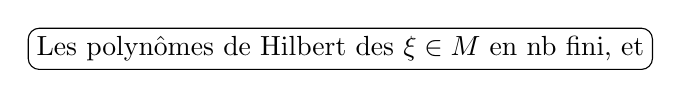
\begin{tikzpicture}\node[draw,rounded corners,inner sep=3pt] {Les polynômes de Hilbert des $\xi\in M$ \unsure{en nb fini, et}};\end{tikzpicture}}
$[\exists$ des faisceaux loc. libres, $A$ et $B$ ($\underline{O}(-n)^N$ si on veut) tels que les $\xi+\gamma(A)$ $(\xi\in M)$ soient décrits par des \uline{faisceaux} loc. libres, quotients de \deleted{un} \inserted{$B$.} \deleted{\unsure{un} faisceau $\underline{O}$ loc. libre ($\underline{O}(-n)^N$ si on veut}$]$.

$(\mathrm{iii})\Longrightarrow(\mathrm{ii})$ trivial, compte tenu que $A,B$ sont quotients de $\underline{O}(-n)^N$ pour $n,N$ convenables,

$(\mathrm{ii})\Longleftrightarrow(\mathrm{i})$ Par la caractérisation des familles limitées

$(\mathrm{ii})\Longrightarrow(\mathrm{iii})$ Car si $G=O(-n)^N/R$, on aura
\[
\xi=\gamma(F)-\gamma(\underline{O}(-n)^N)+\gamma(R)
\]
d'où
\[
\xi+\gamma(\underline{O}(-n)^N)=\gamma(F+R).
\]
Or $\deleted{F+}R$ est un quotient de $\unsure{\underline{O}(-n)^{N'}|\underline{O}(n)^{N'}}$, donc les $F+R$ \uuline{sont} \uline{quotients} d'un
\margin{119}
\scanpage{121}
Supposons \inserted{de plus} $X$ non singulier, et considérons \deleted{des} une partie $M'$ de $\unsure{Z^i(X)_c|Z^i(X)}$ (classes de cycles à $K$-équivalence près---). \inserted{Considérons les} Conditions \deleted{équivalentes} :

i) \deleted{$\unsure{\xi}$} la famille de $M'$ est limitée, i.e. définie par une famille limitée de \uline{cycles} algébriq.

ii) La famille \deleted{de} $M'$ est ``numériquement limitée'' (i.e. un nb fini de classes à équivalence numérique ---) et $\exists$ \deleted{diviseur \unsure{ample|qte}} \inserted{classe} $\unsure{\zeta_0|Z_0}\in Z^i(X)$ telle que les $\deleted{\zeta+\operatorname{cl}(Z_0)}\ \inserted{\zeta_0+\zeta}$ $(\zeta\in M)$ soient ``positifs'' i.e. décrits par des cycles positifs.

iii) \deleted{la famille} \deleted{Il y a une famille limitée de faisceaux loc. libres $F_i$ telle} \inserted{il y a une famille limitée $M\subset K(X)$} telle que $\forall\,\zeta\in M'$, $\exists\,\xi\in M$ \uline{tel que}
\[
(i-1)!\zeta=c^i(\xi)\ \deleted{+\unsure{\zeta+1}}
\]

iv) Il y a une famille limitée $M\subset K^{(i)}(X)$ telle que $M'\subset\operatorname{Img}\text{ de }M$.

v) La famille $M'$ est numériquement limitée.
\margin{120}
\scanpage{122}
\mspage{3}
\deleted{
$M_v(S')=$ ensemble des $g\in G(S')$ tels que $\deleted{\unsure{g\times_S W}}\quad v_{S'}\in g.W(S')$, i.e. tels que $g^{-1}v_{S'}\in W(S')$. Si $v$ est une section de $W$ et non seulement \inserted{de} $V$, alors $M_v$ contient évidemment $N$.

Dans ces explicitations, on n'a pas utilisé le fait que $G,V,W$ étaient représentables (ni que le site sur lequel on travaille est \deleted{\unsure{e}} défini en termes de préschémas ! ). Mais supposons maintenant que $N$ soit représentable et fidèlement plat et quasi-compact sur $S$, et que $G/N$ soit représentable. Lorsque $S$ est le spectre d'un corps, et que $G$ est de type fini sur $k$, on sait que cette hypothèse est \deleted{\illegible{1}} nécessairement satisfaite (Exp VIII 6 et Exp VI). On voit alors sur le diagramme cartésien (xx), utilisant la théorie de la descente fidèlement plate quasi-compacte et le fait que \inserted{$Z\longrightarrow G\times_S V$} est une immersion fermée, que $X$ est représentable (il est obtenu par descente \deleted{\illegible{1}} du sous-préschéma fermé $Z$ de $G\times_S V$ par le morphisme fidèlement plat et quasi-compact $G\times_S V\longrightarrow G/N\times_S V$). Donc le diagramme (D) est un diagramme de morphismes de \deleted{\unsure{schémas}} préschémas sur $S$.

Nous supposons par la suite que $S$ est le spectre d'un corps $k$, et que $G,V,W$ sont de type fini sur $k$. Soit \deleted{\unsure{noté}} $\uline{\mathfrak{n}}$ l'algèbre de Lie de $N$, donc on a $\dim N\leq\operatorname{rang}\uline{\mathfrak{n}}$, l'égalité étant vraie si et seulement si $N$ est lisse sur $k$ (Exp VI). Soit $a\in W(k)$, et considérons le sous-schéma $M_a$ de $G$ défini plus haut, contenant $N$, et isomorphe à $\phi^{-1}(a)$; nous désignerons par $\uline{\mathfrak{m}_a}$ son espace tangent de Zariski en l'élément neutre $e$ de $N$, de sorte qu'on a
\[
(1)\qquad\uline{\mathfrak{n}\subset\mathfrak{m}_a},\quad\deleted{\unsure{\text{donc}}}\quad\dim N\leq\operatorname{rang}\mathfrak{n}\leq\operatorname{rang}\mathfrak{m}_a.
\]
\uline{Lemme 1.1.} \deleted{\unsure{a)}} Avec les notations précédentes:

a) Considérons les conditions suivantes:
\[
(\mathrm{i})\quad\mathfrak{n}=\mathfrak{m}_a\quad\deleted{\illegible{1}}\quad\text{et }N\text{ est lisse sur }k.
\]
}
\margin{?}
\margin{?}
\margin{121}
\scanpage{123}
\unsure{Ceci} posé, on a les implications

\diagram{\begin{tikzcd}[ampersand replacement=\&,column sep=small,row sep=large]
(\mathrm{ii})\arrow[rr,Rightarrow]\&{}\arrow[d,dash]\&(\mathrm{i})\arrow[rr,Leftrightarrow]\&{}\arrow[d,dash,bend left=15]\&(\mathrm{iv})\arrow[rr,Rightarrow]\&{}\arrow[d,dash,bend left=20]\&(\mathrm{iii})\arrow[rr,Rightarrow]\&\& (\mathrm{v})\\
\&\begin{gathered}\text{\unsure{propriété}}\\\text{des familles}\\\text{limitées de}\\\text{faisceaux}\end{gathered}\&\&\begin{gathered}\text{définition}\\\text{de la}\\K\text{-équivalence de}\\\text{cycles}\end{gathered}\&\&\text{R.R.}
\end{tikzcd}}
\margin{122}
\scanpage{124}
\mspage{2}
\deleted{
$Z(S')=$ ensemble des couples $(g,v)\in G(S')\times V(S')$ tels que $v\in g.W_{S'}(S')$.

Par suite, $Z$ est isomorphe au faisceau $G\times_S W$, grâce à l'isomorphisme
\[
G\times_S W\xrightarrow{\sim}Z
\]
défini par $(g,w)\rightsquigarrow(g,g.w)$. Ainsi le diagramme cartésien précédent donne le diagramme cartésien

\diagram{\begin{tikzcd}[ampersand replacement=\&]
\text{(xx)}\&G\times_S W\arrow[r,"q"]\arrow[d,"\lambda"']\&X\arrow[d,"i"]\\
\&G\times_S V\arrow[r]\&G/N\times_S V
\end{tikzcd}}

où on a $\lambda(g,w)=(g,g.w)$, donc $q(g,w)=(g^{\bullet},g.w)$, où $g^{\bullet}$ désigne l'image de $g$ par l'application canonique $G(S')\longrightarrow(G/N)(S')$. On voit enfin sur le diagramme (x) que $Z\longrightarrow X$ fait de $Z$ un fibré principal \deleted{homogène sur} \inserted{de base} $X$ \inserted{et} de groupe $N$ opérant \deleted{\unsure{par}} à droite par $(g,v).n=(gn,v)$, de sorte que \deleted{\unsure{donc}} dans (xx), $q:G\times_S W\longrightarrow X$ fait de $G\times_S W$ un fibré principal de base $X$ et de groupe $N$ opérant \deleted{\unsure{par}} à droite par
\[
(g,w).n=(gn,n^{-1}.w)
\]
Nous \inserted{résumons} \deleted{considérons} \inserted{les principaux morphismes précédents dans} le diagramme suivant :

\diagram{\begin{tikzcd}[ampersand replacement=\&,column sep=large,row sep=large]
\&\&G\times_S W\arrow[d,"q"]\arrow[dr,"\phi"]\&\\
\text{(D)}\&G/N\&X\arrow[l,"p"']\arrow[r,"\psi"']\arrow[d,"i"]\&V\\
\&\&G/N\times_S V\arrow[ul,dashed,"\operatorname{pr}_1"]\arrow[ur,dashed,"\operatorname{pr}_2"']\&
\end{tikzcd}}

où $\psi=\operatorname{pr}_2 i$ et $\phi=\psi q$ \inserted{\begin{tikzpicture}\node[draw,ellipse,inner sep=3pt] {i.e. $\phi(g,w)=g.w$.};\end{tikzpicture}} Si $v$ est une section de $V$ sur $S$, le sous-faisceau $\unsure{X_v}$ de $X$ image inverse de cette section par $\psi$ est donné par

$\unsure{X_v}(S')=$ ensemble des sous-faisceaux $W'$ de $V_{S'}$ qui sont localement conjugués de $W_{S'}$ par $G$, et qui contiennent la section $v_{S'}$ de $V_{S'}$,

tandis que le sous-faisceau $\deleted{\unsure{X_v}}$ de $G\times_S W$ image inverse de $v$ par $\phi$ est \deleted{donné par} isomorphe au sous-faisceau $M_v$ de $G$ \deleted{\unsure{formé}} donné par
}
\margin{$\unsure{M_v}$}
\margin{123}
\scanpage{126}
\diagram{\[
\begin{array}{ll}
1^\circ)&A_{\unsure{r}}^i(X)^a\times A^j(X)^a\ \unsure{\text{---}|\longrightarrow}\ A^{i+j}(X)^a\qquad\uuline{\text{nul}}\\
\Updownarrow&\\
1^\circ\mathrm{bis})&A^i(X)^a\times A^j(\unsure{Y})^a\ \unsure{\text{---}|\longrightarrow}\ A^{i+j}(X\times Y)^a\qquad\uuline{\text{nul}}\\
\Downarrow&
\end{array}
\]
\[
\left\{\begin{array}{ll}
2^\circ)&A_0(X)^a\times A_0(Y)^a\ \unsure{\text{---}|\longrightarrow}\ A_0(X\times Y)^a\qquad\uuline{\text{nul}}\\
\Updownarrow&\\
2^\circ\mathrm{bis})&A_0(X)^a\times A_0(X)^a\longrightarrow A_0(X\times X)^a\qquad\uuline{\text{nul}}\\
\Downarrow&\\
3^\circ)&a,x\in X,\ b,y\in Y\Longrightarrow(x,y)-(x,b)-(a,y)+(a,b)\sim0\\
& (\deleted{a}\in\\
\Updownarrow&\\
3^\circ\mathrm{bis})&\text{Kif-Kif avec }X=Y\\
\Updownarrow&\deleted{A_0(X)^{\unsure{\tau|r}}\longrightarrow\operatorname{Alb}(X)}\\
4^\circ)&\text{Si }A\text{ V.A. --- , \unsure{pr|pour} }x,y\in A\\
&(x+y)-(x)-(y)+(0)\sim_{\unsure{a}}0\\
&\text{i.e. }x\rightsquigarrow(x)-(0)\text{ est un }\uline{\text{hom}}\quad A\ \unsure{\text{---}|\longrightarrow}\ A_0(A)^{\unsure{\tau|a}}\\
&[\text{évid. surjectif !}]\\
\Updownarrow&\\
(4^\circ\mathrm{bis})&\text{Si }A\text{ V.A., }\deleted{\text{\unsure{on a que|pour}}}\text{ l'hom}\\
&A_0(A)^a\longrightarrow A\\
&\text{est un isom.}\quad\begin{gathered}\text{(Alors l'isom réciproque est}\\\text{\unsure{celui envisagé} en }4^\circ\text{)}\end{gathered}\\
\Updownarrow&\\
5^\circ)&\text{Pour }\forall X,\quad A_0(X)^a\longrightarrow\operatorname{Alb}(A),\quad\text{(qui est surj)}\\
&\text{est un }\uline{\text{isom.}}\\
6^\circ)&\text{Pour }X,Y,\text{ l'hom }A_0(X\times Y)^a\ \unsure{\text{---}|\longrightarrow}\ A_0(X)^a\times A_0(Y)^a\\
&\begin{gathered}\inserted{\begin{tikzpicture}[baseline=-.5ex]\node[draw,ellipse,inner sep=2pt] {(qui est surj)};\end{tikzpicture}}\\\longrightarrow\text{bijectif}\end{gathered}\\
6^\circ\mathrm{bis})&\text{Kif Kif avec }X=Y
\end{array}\right.
\]}
\margin{125}
\scanpage{127}
\mspage{25}
\deleted{obtenue par extension du corps de base}
\deleted{
obtient ainsi une ``fibration'' naturelle de l'ouvert dense $U$ des points réguliers de $G$ au dessus du \deleted{\unsure{variété}} préschéma $\deleted{\unsure{U}}\ \unsure{\mathcal{C}|\mathcal{T}}$, les fibres \deleted{géométriques} étant \deleted{\illegible{1}} \inserted{des} ouverts \inserted{denses} de sous-groupes de Cartan des fibres de $G_{\deleted{\unsure{U}}\unsure{\mathcal{C}|\mathcal{T}}}$ (savoir les ouverts des points réguliers dans $G$). \deleted{modulo extension du corps de base.} On trouve par exemple\inserted{: le résultat suivant (qui sera considérablement précisé dans l'exposé suivant):}

\uline{Corollaire 3.3.} Soient $G$ un groupe algébrique lisse connexe \deleted{affine} sur le corps $k$, $\unsure{\mathcal{C}|\mathcal{T}}$ le schéma des tores maximaux de $G$ ($\simeq$ le schéma des sous-groupes de Cartan de $G$). Alors le corps des \deleted{fonctions} fonctions $k(G)$ \inserted{de $G$} est isomorphe au corps de fonctions d'un groupe algébrique lisse connexe affine nilpotent $C$ sur le corps des fonctions $k(\unsure{\mathcal{C}|\mathcal{T}})$ de $\unsure{\mathcal{C}|\mathcal{T}}$, savoir $C=\deleted{\unsure{a}}$ ``le sous-groupe de Cartan générique de $G$''. Si \deleted{$k$ est de rang unipotent nul, i.e.} \inserted{$G$ est affine de rang unipotent nul, i.e. si} les sous-groupes de Cartan \inserted{de $G_{\bar{k}}$} sont des tores, alors $k(G)$ est une extension unirationnelle de $k(\unsure{\mathcal{C}|\mathcal{T}})$.

Bien entendu, par sous-groupe de Cartan générique de $G$, on entend (par abus de langage) le sous-groupe de Cartan de $G_{k(\unsure{\mathcal{C}|\mathcal{T}})}$ fibre générique de $X$ au dessus de $\unsure{\mathcal{C}|\mathcal{T}}$. Il n'y a plus qu'à prouver la dernière assertion de 3.3., qui est contenue dans le \inserted{résultat bien connu suivant (dû à Chevalley):}

\deleted{\uline{Lemme 3.4.} Soient $k$ un corps, $T$ un tore sur $k$, $k(T)$ le corps des fonctions rationnelles sur $T$, alors $k(T)$ est une extension unirationnelle de $k$, i.e. est contenue dans une extension transcendante pure de $k$.

Soit en effet $k'$ une extension finie \deleted{\illegible{1}} séparable de $k$ \deleted{\unsure{a}} qui splitte $T$ (Exp X 1.4.), alors \deleted{\unsure{le}} $T\otimes_k k'$ est une variété rationnelle i.e. \deleted{\unsure{isomorphe bir}} admet un ouvert dense isomorphe à un ouvert dense de l'espace euclidien $E_k^n$, donc
\[
T'=\prod_{\operatorname{Spec}(k')/\operatorname{Spec}(k)}T_{k'}/\operatorname{Spec}(k')
\]
est une variété rationnelle (car admet un ouvert dense isomorphe à un ouvert dense de $\prod_{\operatorname{Spec}(k')/\operatorname{Spec}(k)}E_{k'}^n$, qui est isomorphe à l'espace \deleted{\unsure{non}} eucli-
}
}
\margin{Conserver le texte ci-contre, barré par erreur.}
\margin{126}
\scanpage{128}
\diagram{\[\begin{array}{cc}X&Y\\a&b\end{array}\]}
\[
X\times Y=Z\qquad\qquad A\times A\ \unsure{\text{---}|\longrightarrow}\ A
\]
\[
\underbrace{(\bar\zeta\times b)}_{\unsure{\sim0}}\times\underbrace{(a\times\zeta')}_{\sim0}\quad\text{dans }Z\times Z=X\times Y\times X\times Y
\]
\[
(\bar\zeta\times\zeta')\times(b\times a)
\]
\margin{\rotatebox{180}{$\displaystyle\frac{X^2}{R}(S')\ne\frac{X^2(S')}{R(S')}\quad\unsure{\infty}$}}
\figure{\begin{tikzpicture}[scale=.65]
\draw (4,3.7) .. controls (2,4.2) and (.2,4.3) .. (.7,3.6);
\draw (3.6,4) -- (3.5,.5);
\draw (1.8,2.7) circle (.04);\draw (3,2.7) circle (.05);
\draw (1.7,1.5) circle (.04);\draw (3,1.5) circle (.05);
\draw (-2,.3)--(1.1,1.15);
\draw (-2.1,.6) .. controls (-2.8,-.3) and (-1.4,.05) .. (-.9,.45)
.. controls (-.2,.95) and (.05,.75) .. (-.3,.55)
.. controls (-1.1,.2) and (-.6,1.0) .. (-.05,1.0)
.. controls (.7,1.55) and (1.4,1.65) .. (1.35,.9);
\end{tikzpicture}}
\[
\deleted{\sum\unsure{\lambda|A}(x,y)}\qquad
\deleted{(x,y)}\ \sum\unsure{n|u}_{x,y}(x,y)
\]
\margin{\rotatebox{180}{$\begin{array}{l}\unsure{a}^{-1}(ab)=b\\a(a^{-1}b)=b\\(ba)a^{-1}=b\\(ba^{-1})a=b\end{array}$}}
\[
3\Longrightarrow4
\]
\deleted{$\unsure{A}$}
\diagram{\begin{tikzcd}[ampersand replacement=\&,column sep=large]
A\arrow[r,"\uline{\text{hom surjectif}}"]\&A_0(A)^{\tau}\arrow[l,bend left=35,"\uline{\text{hom surjectif}}"]
\end{tikzcd}}
\[
A\longrightarrow A_0(A)^\tau\qquad\text{est bij.}
\]
\[
\unsure{\zeta}
\]
\figure{\begin{tikzpicture}
\node[anchor=center,inner sep=8pt] (d) at (0,0) {\diagram{\begin{tikzcd}[ampersand replacement=\&,column sep=large,row sep=large]
\&{[2,2\mathrm{bis},3,3\mathrm{bis}]}\arrow[r,Leftrightarrow,"\boxed{\unsure{\text{via les corrtces}|\text{via les courbes}}}"]\&{[4,4\mathrm{bis}]}\arrow[r,Rightarrow,"\deleted{\text{\unsure{th. de Weil}}}"]\arrow[dl,Rightarrow,"?"']\&{[5]}\\
{[6^\circ,6\mathrm{bis}]}\arrow[ur,Rightarrow]\&\deleted{\unsure{(\varphi\times\psi)\ \text{épimorphe}}}\&\&\\
|[draw,circle]|5^\circ\arrow[u,Rightarrow]\&\unsure{3^\circ}\arrow[uu,Rightarrow,"\deleted{\text{\unsure{th. de Weil}}}"']\&\&
\end{tikzcd}}};
\draw[rounded corners] (d.north west) rectangle ([yshift=1.1cm]d.south east);
\node[anchor=east] at ([xshift=-8pt]d.west) {$\operatorname{Alb}(X\times Y)$};
\draw ([xshift=-15pt,yshift=-5pt]d.west) .. controls (-6,-2.7) and (1,-1.5) .. ([xshift=8pt]d.east)
.. controls (7,4.4) and (1,3.5) .. ([xshift=-12pt,yshift=2pt]d.west);
\draw ([xshift=-4pt]d.south west) .. controls (-5,-4) and (-2,-3.8) .. ([xshift=-20pt,yshift=-5pt]d.south);
\end{tikzpicture}}
\[
A_0(\unsure{X\times Y})\ \unsure{\text{---}|\longrightarrow}\ A_0(\qquad
\]
\[
A_0(X)\times A_0(Y)\longrightarrow A_0(X\times Y)
\]
\diagram{\begin{tikzcd}[ampersand replacement=\&]
\times\&\\
A_0(X\times Y)^\tau\arrow[r,dash]\arrow[d,dash]\&A_0(X)^\tau\times A_0(Y)^\tau\\
\unsure{\operatorname{Alb}(X)\times\operatorname{Alb}(Y)}.\quad(\&
\end{tikzcd}}
\[
\deleted{x,y}\quad\bar x,y\qquad\deleted{\varphi(x)-\varphi(a)}
\]
\[
\deleted{x,a}\quad\deleted{x-a}\qquad\varphi(x)-\varphi(a),\quad\psi(y)-\psi(b)
\]
\[
(x,y)-(x,b)-(a,y)+(a,b)
\]
\[
x-x-a+a
\]
\margin{127}
\scanpage{129}
\mspage{24 bis}
\deleted{
\deleted{
$G_b$, où $b\in\Gamma(G,O_G)$ est la section définie dans 2.7. (NB on \unsure{décomposera} $S$ en le préschéma somme des préschémas $S_{n,\rho}$, sur chacun desquels $G$ est de dimension relative $n$ et de rang \deleted{réductif} nilpotent $\rho$, et on construit $b$ séparément sur chacun des $G\vert S_{n,\rho}$). D'autre part, comme $\unsure{\Psi|\psi}^{-1}(U)$ et $U$ sont lisses donc plats localement de présentation finie sur $S$, pour vérifier que $\psi$ induit un isomorphisme $\psi^{-1}(U)\longrightarrow U$, il suffit de le vérifier fibre par fibre, \inserted{(SGA I 5.7.)} ce qui nous ramène au cas où $S$ est le spectre d'un corps, que l'on peut supposer algébriquement clos. Il existe alors un sous-groupe de Cartan $C$ de $G$, et si $N$ est le normalisateur, on sait \deleted{\unsure{que}} par le théorème de conjugaison que $\mathcal{C}$ s'identifie à $G/N$, et le morphisme $\psi:X\longrightarrow G$ n'est autre que celui défini dans le N° 2. On conclut alors par 2.6. b). Enfin, \deleted{il est aussi} cela montre aussi que $U$ est le \uline{plus grand} ouvert \inserted{$V$} de $G$ tel que $\psi^{-1}(V)\longrightarrow V$ soit un isomorphisme, car \deleted{il suffit de le vérifier encore dans} pour vérifier $V\subset U$, il suffit de le vérifier fibre par fibre.
}

\uline{Corollaire 3.2.} Sous les conditions de 3.1., soit $g$ une section régulière de $G$, i.e. telle que pour tout $s\in S$, $g(s)$ soit un point régulier de $G_s$. Alors il existe un et \inserted{un} seul sous-groupe de Cartan $C$ de $G$ \deleted{contenant $g(S)$} tel que $g$ soit une section de $C$.

En effet, l'hypothèse sur $g$ signifie que $g$ est une section de $U$, et la conclusion qu'il existe une unique section de $X$ qui la relève, ce qui \deleted{\unsure{revient}} n'est qu'une autre façon d'exprimer que $\psi^{-1}(U)\longrightarrow U$ est un isomorphisme.

Notons maintenant que l'ouvert $\psi^{-1}(U)$ du sous-groupe de Cartan $X$ de $G_{\deleted{\unsure{X}}\mathcal{C}}$ n'est autre que l'ouvert de $X$ formé des points de $X$ qui sont réguliers dans $G_{\deleted{\unsure{X}}\mathcal{C}}$ (par quoi on entend: réguliers dans leur fibre). On
}
\margin{\begin{tikzpicture}\node[draw,ellipse] {indice $\mathcal{C}$};\end{tikzpicture}}
\margin{128}
\scanpage{131}
\diagram{\begin{tikzcd}[ampersand replacement=\&]
Z\subset X\times S\arrow[d,dash]\\
\text{cycle d'incidence}
\end{tikzcd}}
\[
Z^i(Y
\]
\diagram{\begin{tikzcd}[ampersand replacement=\&,column sep=large,row sep=large]
\&P(N)\arrow[dl,dash,"\text{codim }j"']\\
C\subset X\&X'\arrow[l,"\text{éclaté}"']\arrow[d]\\
\&S
\end{tikzcd}}
\diagram{\begin{tikzcd}[ampersand replacement=\&,column sep=large,row sep=large]
\&C\times S\arrow[d,phantom,"\rotatebox{90}{$\simeq$}" description]\&\\
C\arrow[d,"\text{codim }j+1"']\&P(N)\arrow[l]\arrow[d,"\alpha"]\arrow[r,leftrightarrow]\&C_y\arrow[d,"\alpha_y"',"\text{codim }j"]\\
X\&X'\arrow[l,"f"']\arrow[r,leftrightarrow,"i'_y"']\arrow[d]\&Y(y)\arrow[d]\arrow[ll,bend left=40,"i_y"']\\
\&S\arrow[d,dash]\&y\text{ pt gén}\arrow[l]\\
\&\uline{\text{variété \unsure{rationnelle}}}\&
\end{tikzcd}}
\[
y_y=i_y^{\prime *}(y')
\]
\[
f_*(y')=x
\]
\[
i_y^*(x)=i_y^{\prime *}(f^*f_*(y'))\qquad f^*f_*y'=y'+\alpha_*(u)
\]
\[
\begin{aligned}
i_y^*(x)&=i_y^{\prime *}(y')+i_y^{\prime *}(\alpha_*(u))\\
&=y'+\alpha_{y*}(u_y)
\end{aligned}
\qquad\begin{gathered}\text{Or }u_y=u\\u\in A(C)\end{gathered}
\]
Donc
\[
\boxed{A(Y(y))=\operatorname{Im}A(X)+\operatorname{Im}A(C)}.
\]
\unsure{i.e.}
\[
A^i(Y(y))=\operatorname{Im}A^i(X)+\operatorname{Im}\unsure{\ell|\sum}A^{i-j}(C)
\]
\margin{130}
\scanpage{132}
\figure{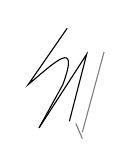
\begin{tikzpicture}[scale=.55]
\draw (0,0)--(-.9,-1.3).. controls (-.3,-.8) and (.3,-.2) ..(-.1,-1.3)--(-.65,-2.3);
\draw (-.65,-2.3)--(.45,-.6)--(.05,-2.15);
\draw[gray] (.85,-.55)--(.35,-2.4);
\draw[gray] (.2,-2.2)--(.35,-2.55);
\end{tikzpicture}}
\figure{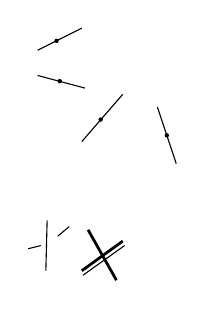
\begin{tikzpicture}[scale=.8]
\draw (0,2)--(.7,2.35);\fill (.3,2.15) circle(.035);
\draw (0,1.6)--(.75,1.4);\fill (.35,1.51) circle(.035);
\draw (.7,.55)--(1.35,1.3);\fill (1, .9) circle(.035);
\draw (1.9,1.1)--(2.2,.2);\fill (2.05,.65) circle(.035);
\draw (-.15,-1.15)--(.05,-1.1);\draw (.15,-.7)--(.13,-1.5);\draw (.32,-.95)--(.5,-.8);
\draw[line width=1pt] (.8,-.85)--(1.25,-1.65);\draw[line width=1pt](.7,-1.5)--(1.35,-1.03);\draw(.72,-1.57)--(1.38,-1.1);
\end{tikzpicture}}
\rotatebox{90}{$\begin{array}{ll}
\deleted{\unsure{k[x^i|k[x}}&\unsure{x^2|x^3}-y^2\\
&k[y]\qquad\unsure{12,13|p^2,p^3}\\
&k[x,y]/xy
\end{array}$}

\rotatebox{180}{\begin{tabular}{c}
INSTITUT\\
DES HAUTES ÉTUDES SCIENTIFIQUES\\
\rule{1cm}{.4pt}
\end{tabular}}
\margin{131}
